\appendix
\section{Appendix}
\subsection{The derivation of FLOPs w.r.t the vocabulary size for the Approach 2}
\label{append:df_dv}
Here we provide the detailed process of how we compute the extreme point of FLOPs $C$ with respect to $V$. From \citet{kaplan2020scaling}, we know that:
\begin{equation}
\label{eq:flops}
    C \approx 6ND \approx 6(N_{\rm nv}+Vd)Hf(V).
\end{equation}

We then compute the derivative $\frac{\partial C}{\partial V}$ as follows:
\begin{align*}
% \label{eq:df_dv_full}
\frac{\partial C}{\partial V} &= \frac{\partial}{\partial V} \left[ 6(N_{\rm nv} + dV)H \left( f(V) \right) \right] \\
&= \frac{\partial}{\partial V} \left[ 6(N_{\rm nv} + dV)H \left( a(\log(V))^2 + b\log(V) + c \right) \right] \\
&= 6H \Bigg[ (N_{\rm nv} + dV) \frac{d}{dV} \left( a(\log(V))^2 + b\log(V) + c \right) \\
&\quad\quad\quad\quad + \left( a(\log(V))^2 + b\log(V) + c \right) \frac{d}{dV}(N_{\rm nv} + dV) \Bigg] \\
&= 6H \Bigg[ (N_{\rm nv} + Vd) \frac{2a \log(V) + b}{V} + \left(a (\log(V))^2 + b \log(V) + c\right)d \Bigg].
\end{align*}

The solution of $\frac{\partial C}{\partial V}=0$ corresponds to the minimum point of the FLOPs. Since the variable $V$ in this equation is not separated conveniently, we use a numerical search method, specifically \texttt{scipy.optimize.fsolve}, to find the solution. 

\paragraph{Example demonstration}
\autoref{fig:df_dv_example} illustrates the relationship between the derivative of FLOPs with respect to the vocabulary size $V$ and $V$ itself. Setting $V$ as the solution to $\frac{\partial C}{\partial V}=0$, we find the point at which FLOPs are minimized. As depicted in \autoref{fig:df_dv_example} (right), the FLOPs budget is fixed, and we observe how the training character varies with $V$. Notably, at the optimal vocabulary size $V$, the model expends the maximum number of training characters for a given budget. This observation provides insight into why an optimal vocabulary size exists for a given FLOPs budget.




\begin{figure}[htbp]
\centering
\begin{subfigure}[b]{0.32\textwidth}  
    \centering
    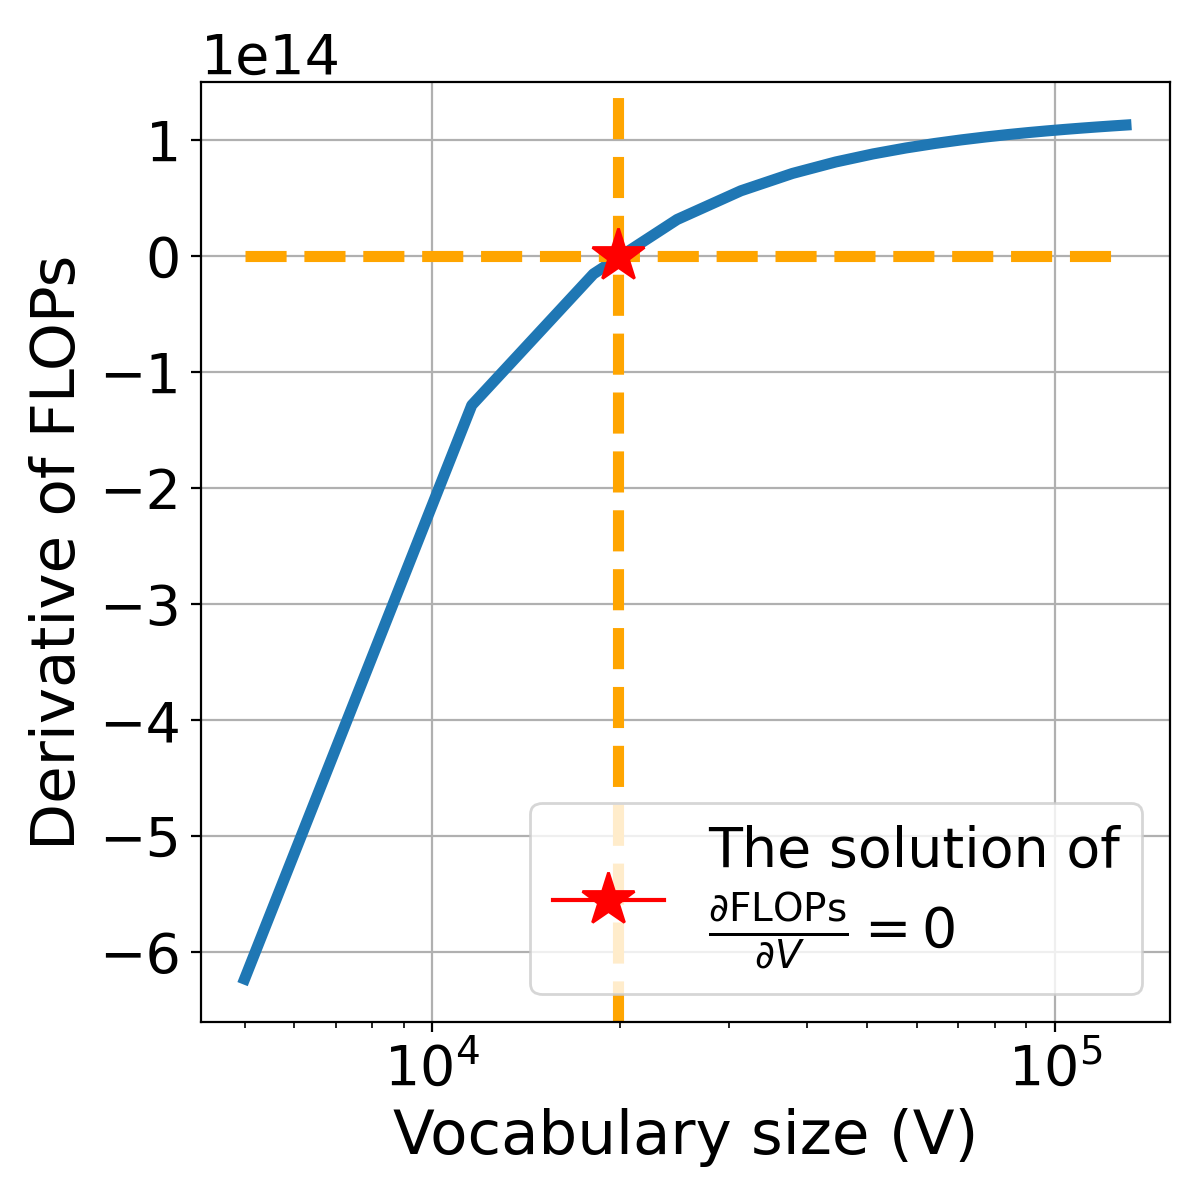
\includegraphics[width=\textwidth]{figures/derivative.png}
\end{subfigure}
\begin{subfigure}[b]{0.32\textwidth}  
    \centering
    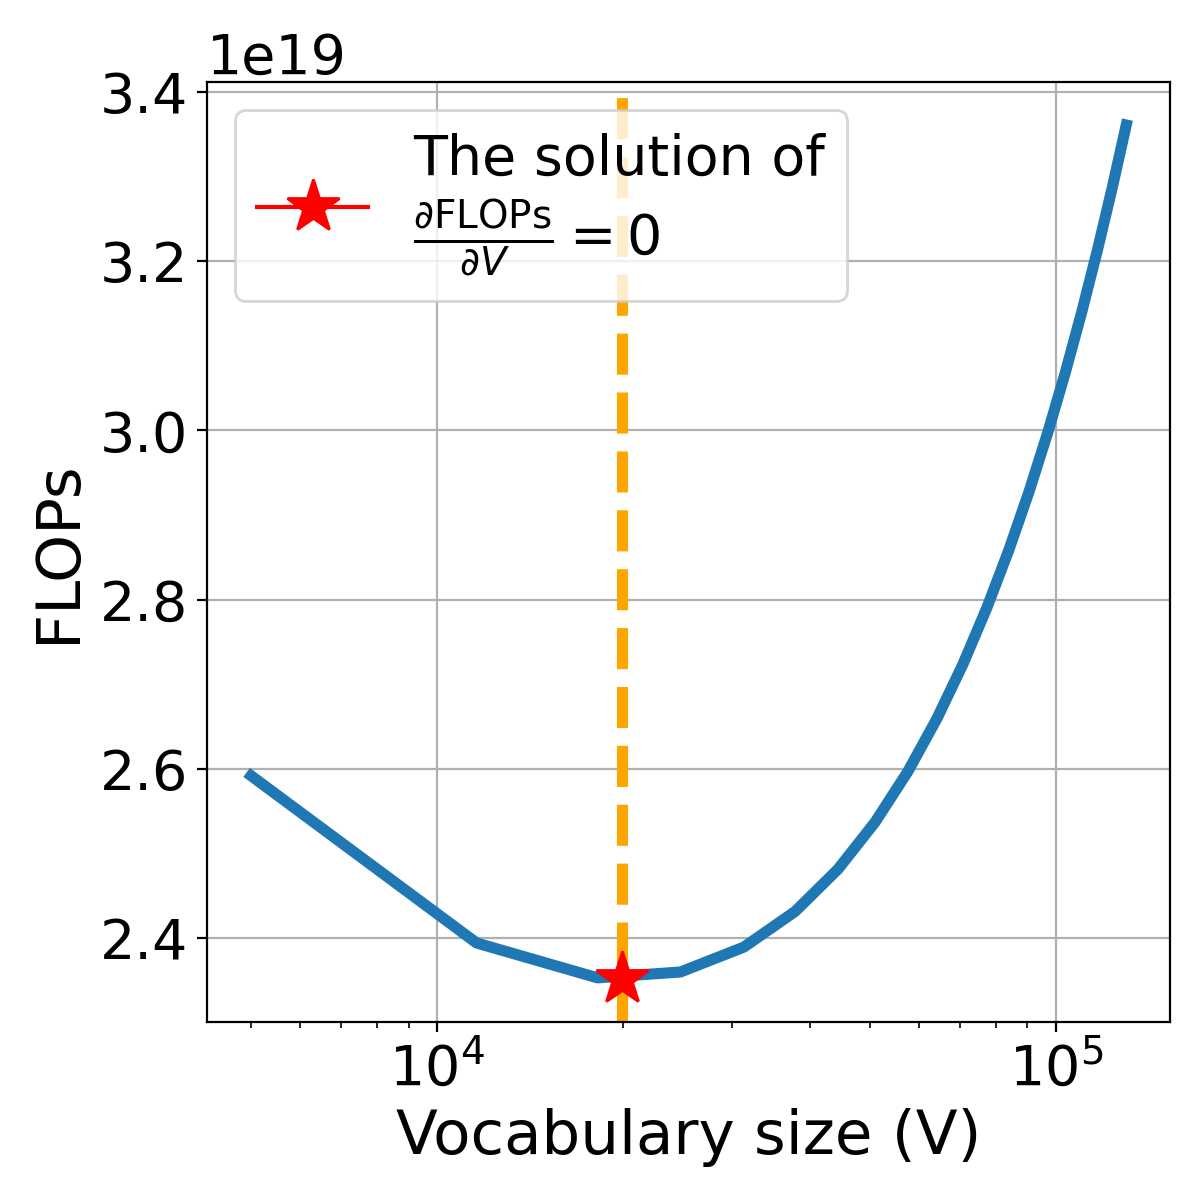
\includegraphics[width=\textwidth]{figures/derivative-flops.png}
\end{subfigure}
\begin{subfigure}[b]{0.32\textwidth}  
    \centering
    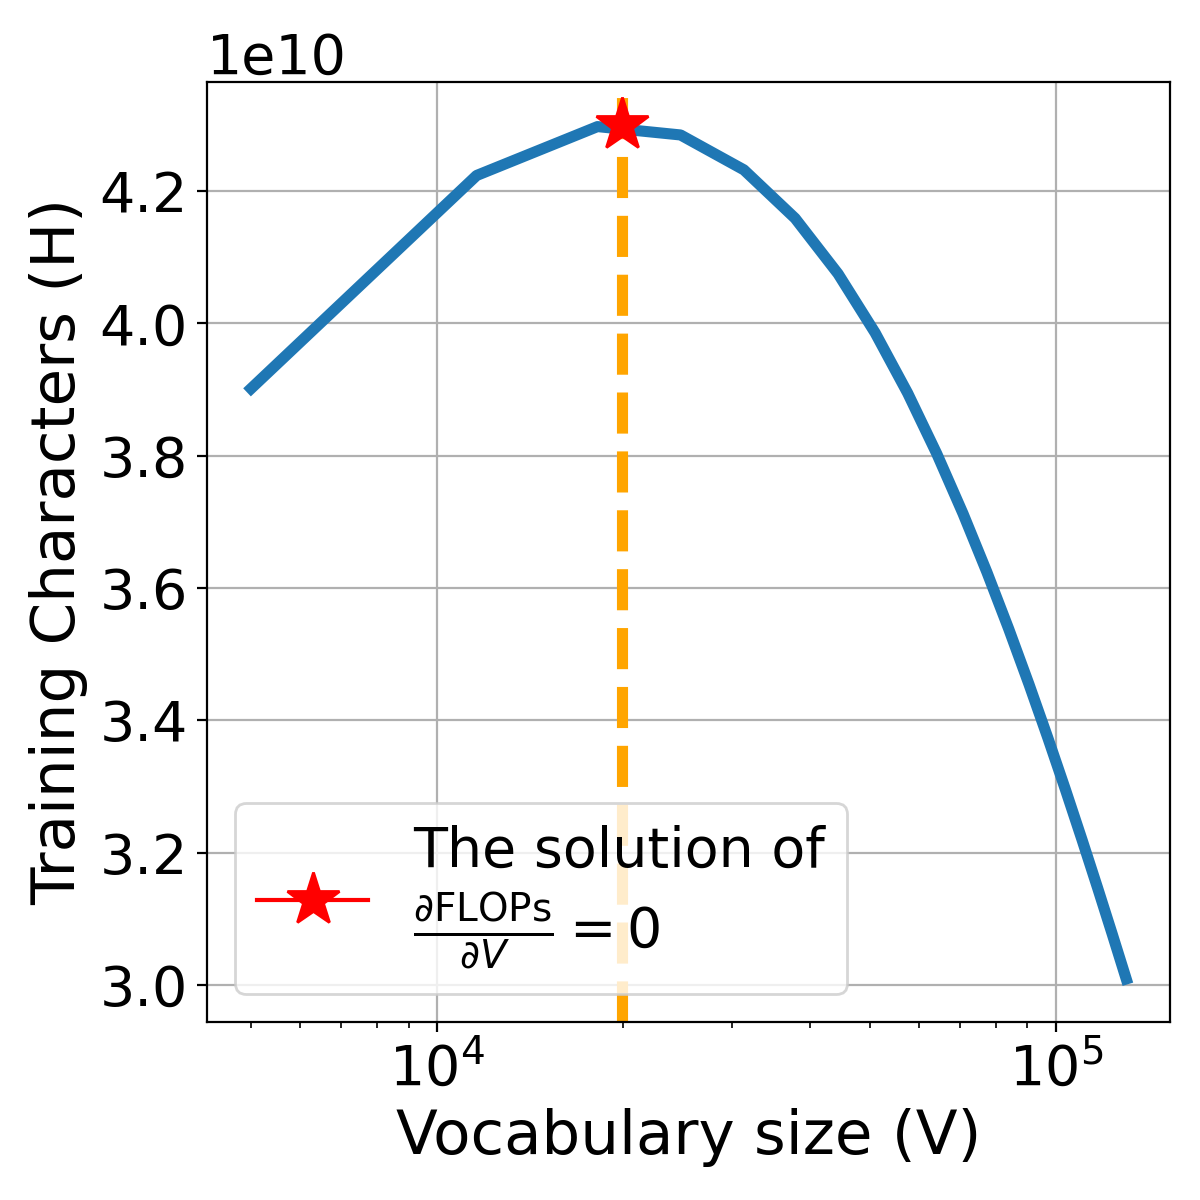
\includegraphics[width=\textwidth]{figures/derivative-H.png}
\end{subfigure}
\caption{\textbf{Left:} The curve of the derivative of FLOPs with respect to vocabulary size  $V$. The curve of  $\frac{\partial C}{\partial V}$ increases as $V$ increases, and the FLOPs reach a minima at the solution of $\frac{\partial C}{\partial V}=0$. \textbf{Middle:} The curve of FLOPs with respect to vocabulary size $V$, where $V$ reaches its optimal point $V$.
\textbf{Right:} The curve of training characters with a given FLOPs budget.
Take $N_{\rm nv}=302M$ and $H=43B$ as an example. 
The FLOPs budget is decided by the $N_{\rm nv}$, $H$ and the predicted $V$.}
\label{fig:df_dv_example}
\end{figure}


\subsection{The derivation of loss w.r.t the vocabulary size in Approach 3}
\label{append:dloss_dv} 
Here we provide how we derive the loss w.r.t the vocabulary size  given a FLOPs budget $C$ in Approach 3. After substituting the $[Hf(V)]$ with the $C/(6(N_{\rm nv} + N_v)$ based on \autoref{eq:flops}: 

\begin{equation}
    \mathcal{L}_u = -E + \frac{A_1}{N_{\rm nv}^{\alpha_1}} +\frac{A_2}{N_v^{\alpha_2}}+ \frac{B}{[C/(6(N_{\rm nv} + N_v)]^{\beta}}.
\end{equation}

The loss is solely dependent on the $N_v=Vd$, given a $N_{\rm nv}$. The derivative w.r.t. $V$ is:
\begin{align*}
 \frac{\partial \mathcal{L}_u}{\partial V} &=
 \frac{\partial}{\partial V} \left( \frac{A_2}{(Vd)^{\alpha_2}} \right) + \frac{\partial}{\partial V} \left( \frac{B}{\left(\frac{C}{6(N_{\rm nv} + Vd)}\right)^{\beta}} \right)\\
 &=
 -\alpha_2 \frac{A_2 d}{(Vd)^{\alpha_2 + 1}} + \beta \frac{B \frac{C d}{6(N_{\rm nv} + Vd)^2}}{\left(\frac{F}{6(N_{\rm nv} + Vd)}\right)^{\beta + 1}}.
\end{align*}

The solution of $\frac{\partial \mathcal{L}_u}{\partial V}=0$ corresponds to the optimal $V$. Similar with Approach 2, we use \texttt{scipy.optimize.fsolve} to find the solution. 




\subsection{More visualizations for the analyses: Why the optimal vocabulary size is bounded by the compute}
\label{append:motivation}

\paragraph{Word embeddings in a large vocabulary are hard to learn when FLOPs are constrained} 
\begin{figure}[htbp]
\centering
\begin{subfigure}[b]{0.31\textwidth}  
    \centering
    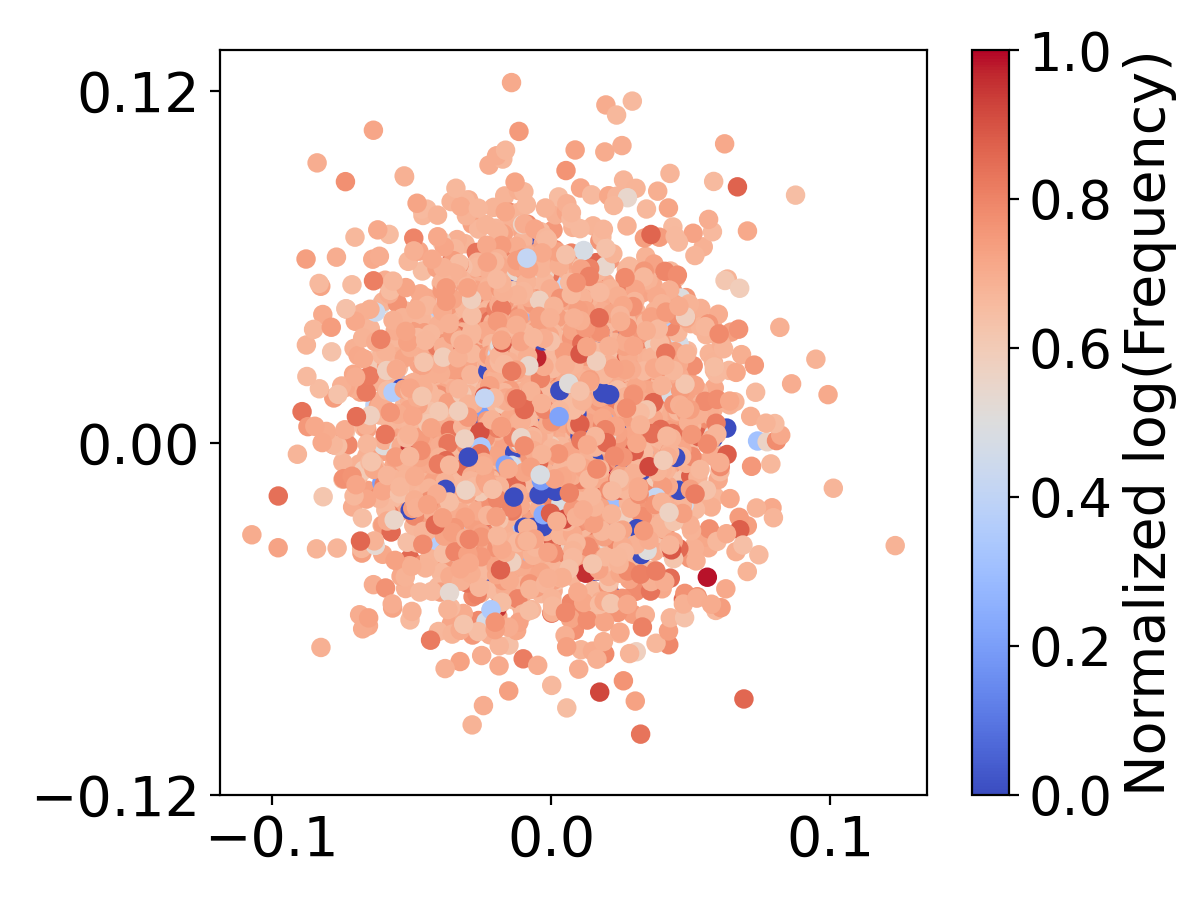
\includegraphics[width=\textwidth]{figures/110m_isoflops_word_dis-V4096-avg_euclidean_dis-0.000.png}
    \label{fig:word-embedding-4k}
\end{subfigure}
\begin{subfigure}[b]{0.31\textwidth}  
    \centering
    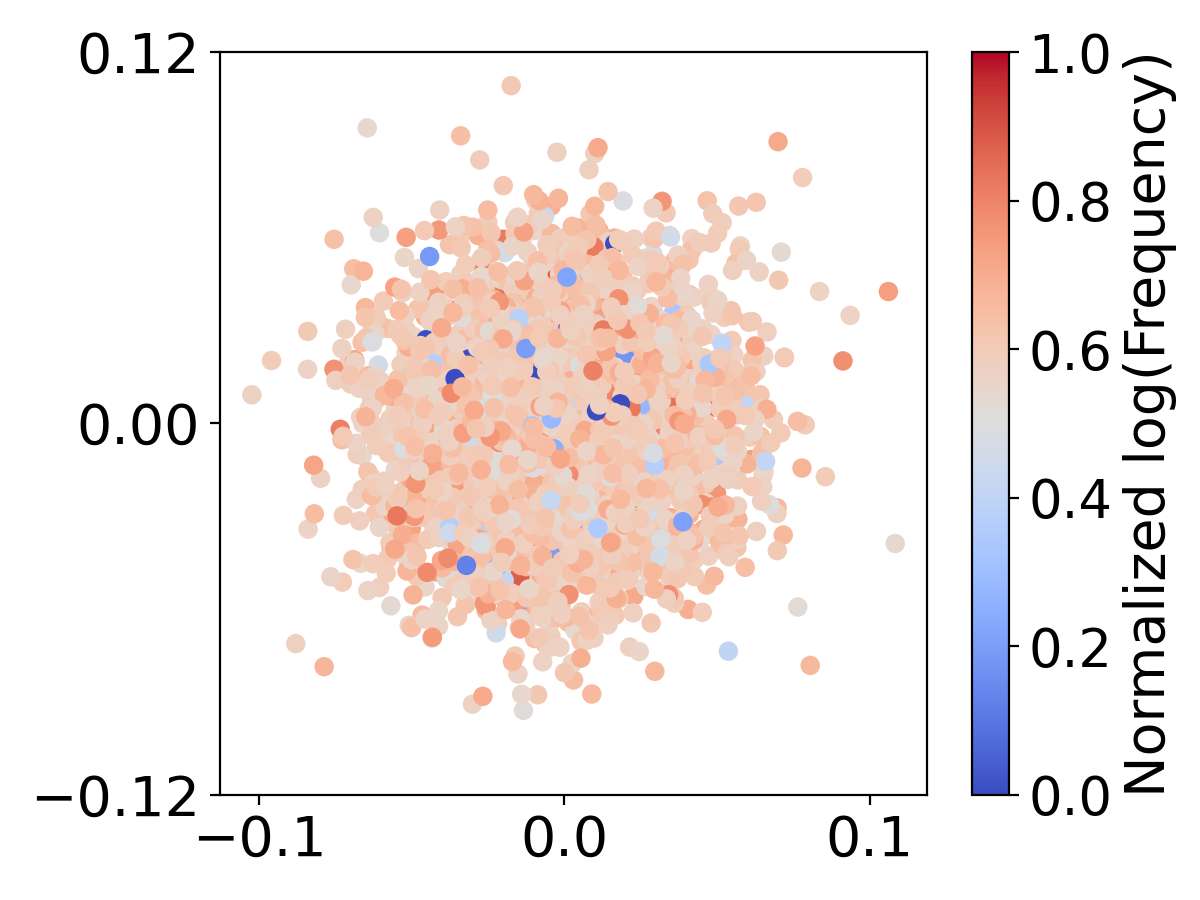
\includegraphics[width=\textwidth]{figures/110m_isoflops_word_dis-V16384-avg_euclidean_dis-0.000.png}
    \label{fig:word-embedding-16k}
\end{subfigure}
\begin{subfigure}[b]{0.31\textwidth} 
    \centering
    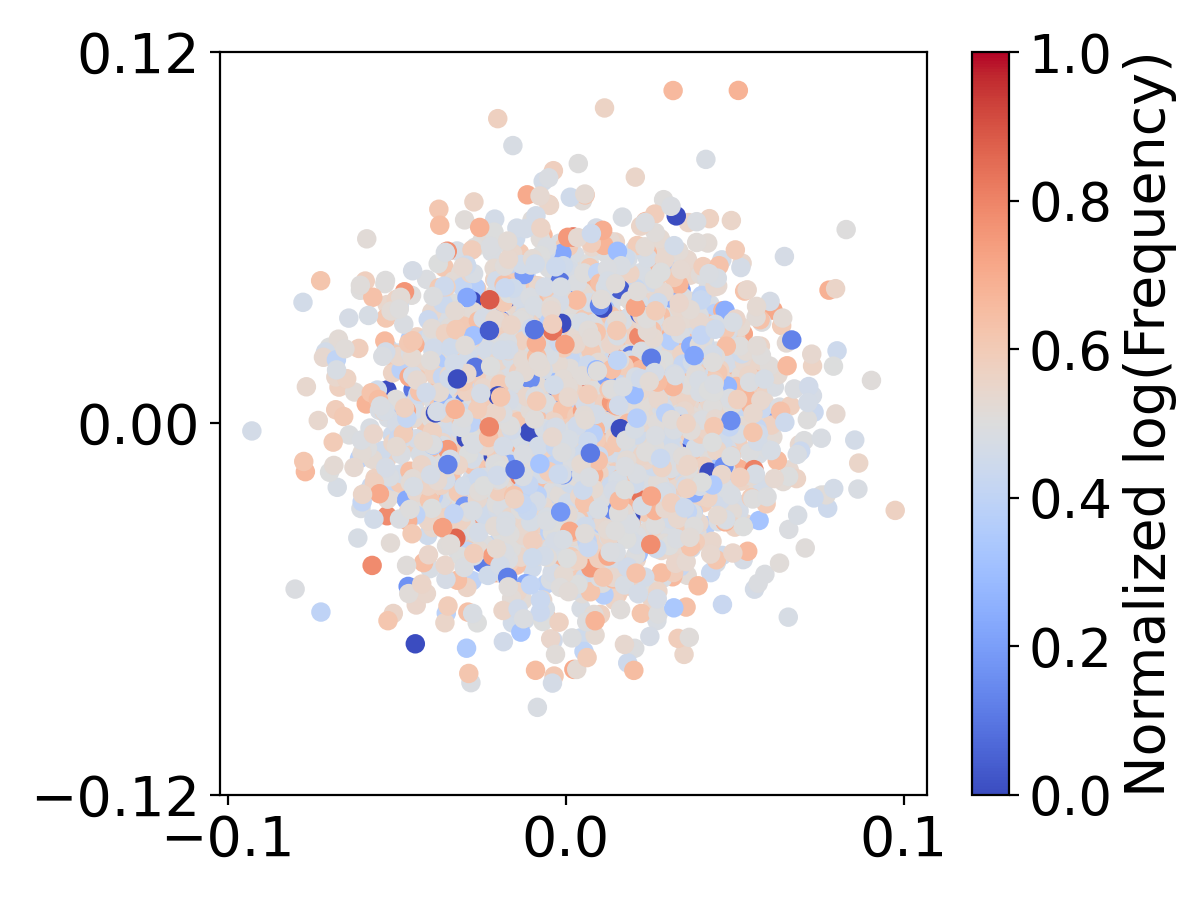
\includegraphics[width=\textwidth]{figures/110m_isoflops_word_dis-V64512-avg_euclidean_dis-0.000.png}
    \label{fig:word-embedding-64k}
\end{subfigure}
\caption{The SVD plots of the learned word embedding for V=4$K$ (left), V=16$K$ (middle) and V=64$K$ (right) for a model with $N_{\rm nv}=85M$. Different colors represent different log frequencies.}
\label{fig:word-embedding}
\end{figure}

Previous studies have shown embeddings suffer from representation degradation, where low-frequency word embeddings cluster together due to limited parameter updating \citep{gao2019representation}. In \autoref{fig:word-embedding}, we visualize how the word embeddings distribute using different vocabulary sizes. We use the average Euclidean distance among all the embeddings, $\mathcal{D}_{avg}$, to quantify the degree of clustering, which is 1.067, 1.011, and 0.952 for $V=4K$, $V=16K$ and $V=64K$, respectively. Larger vocabularies ($64K$) lead to more clustering of embeddings, especially for infrequent words. This clustering suggests that they have been insufficiently trained. Conversely, a small-sized vocabulary ($4K$) and middle-sized vocabulary ($16K$) display a more dispersed distribution of embeddings. These observations suggest that there exists an optimal vocabulary size that balances lexicon coverage and sufficient updating of word embedding. Language models with large vocabulary sizes may have better lexicon coverage, but on the other hand, hinder the model's ability to sufficiently update the word embeddings, especially for low-frequency words.


\subsection{Exploration of Larger Range of Vocabulary Sizes}
\begin{figure}[htp]
  \centering
  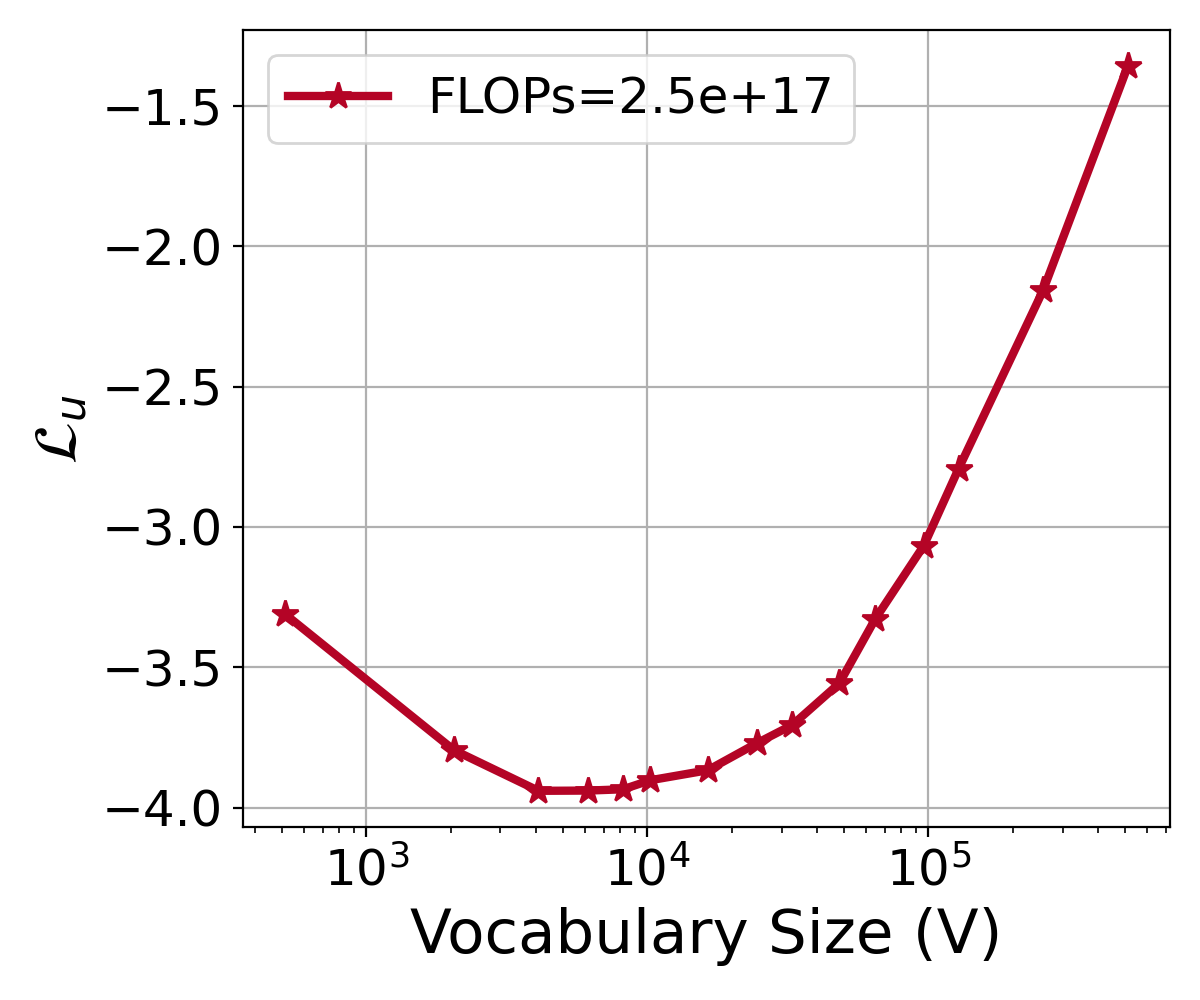
\includegraphics[width=0.5\textwidth]{figures/motivation-ISOFlops-V-loss-more.png}
  \caption{
  Loss curves with larger range of vocabulary sizes (from [4K, 96K] to [0.5K, 512K]), given a certain FLOPs budget. The model performance degrades consistently when the vocabulary size goes beyond the optimal configuration.}
  \label{fig:larger-v}
\end{figure}

Because of computational resource constraints, the vocabulary sizes we used to fit the scaling laws are in the range of 4K to 96K. This range is sufficient to fit, because the optimal vocabulary sizes for all the training configurations we used fall in this range.

To further verify that there is always an optimal vocabulary size holds for a larger range of vocabulary lists, we increase the range of vocabulary sizes from 0.5K to 512K, with the $N_{\rm nv}$ fixed as 33M. As depicted in the \autoref{fig:larger-v}, the model's performance declines consistently as the vocabulary size increases beyond the optimal configuration. This figure shows loss curves for vocabulary sizes up to 512K, given a specific FLOPs budget. The data indicates a consistent degradation in model performance with the vocabulary size away from the optimal one. It suggests that there is a critical point beyond which the model's efficiency in handling the vocabulary diminishes. This exploration underscores the importance of carefully selecting the vocabulary size to maintain optimal model performance within the constraints of a given computational budget.


\subsection{The Vocabulary-insensitive Metric: $\mathcal{L}_u$ and BPC}
\label{append:bpc}
\begin{figure}[htp]
  \centering
  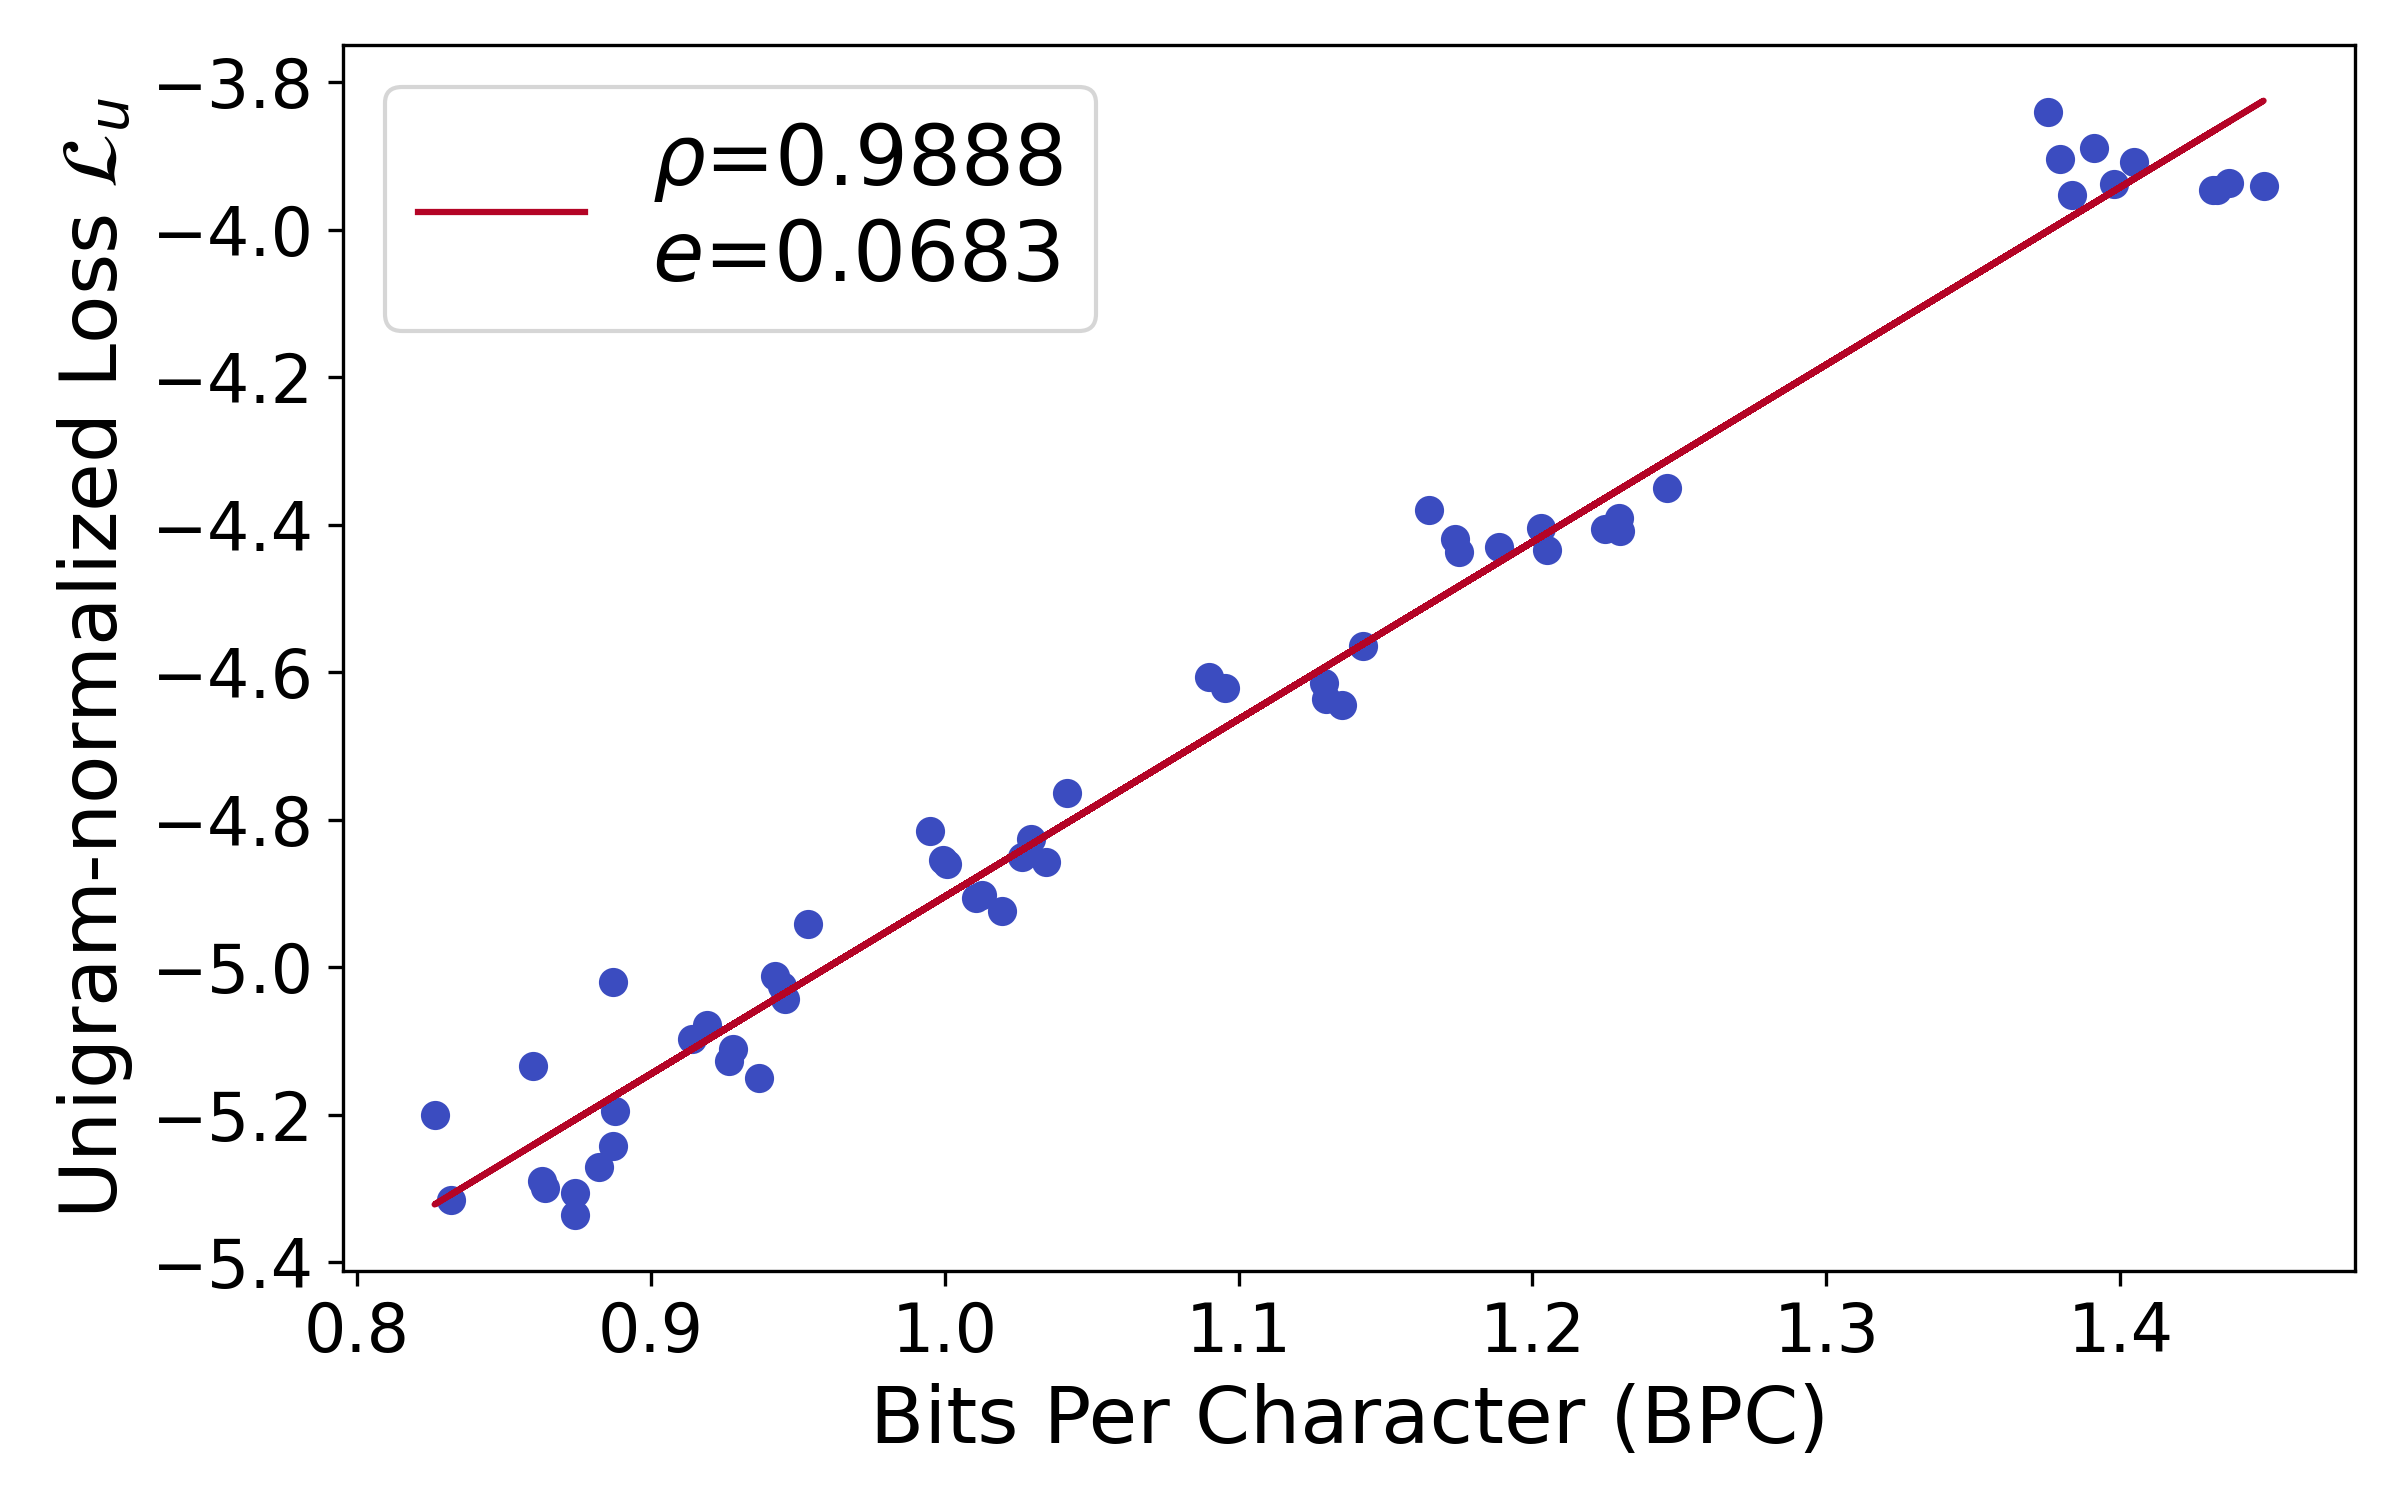
\includegraphics[width=0.75\textwidth]{figures/bpc_lossu_fit.png}
  \caption{
  Correlation between the unigram-normalized loss $\mathcal{L}_u$ and BPC, where $\rho$ and $e$ denote the Pearson correlation coefficient and the root mean square error of the linear fit, respectively.}
  \label{fig:bpc}
\end{figure}
BPC reflects the ability to compress external text corpora \citep{compression2024}, while the unigram-normalized loss reflects the model's ability to predict tokens normalized by the token frequency.   \autoref{fig:bpc} shows the relationship between the Unigram-normalized Loss $\mathcal{L}_u$ and Bits Per Character (BPC) with a linear fit. We select the models of the final training steps
for each $N_{nv}$ and each vocabulary size. The high correlation coefficient ($\rho$ = 0.9888) and low error ($e$ = 0.0683) indicate a strong linear relationship between these two metrics generally.  However, it exists slight different trends due to different normalizations.

\subsection{More Explanations about Why We Separate Vocabulary Parameters from the total Model Parameters}
\label{append:model_growing}
Traditionally, scaling up model parameters in language models has been approached in two ways: increasing depth (i.e., the number of layers) or width (i.e., the hidden size). While extensive research has been conducted on these methods, current empirical practices often involve expanding both simultaneously~\citep{tay-etal-2023-scaling}. This approach, however, may overlook crucial distinctions in how different parameters benefit from these expansions.

Non-vocabulary parameters can benefit from increases in both depth and width, allowing for more complex hierarchical representations and broader feature capture.
In contrast, vocabulary parameters, associated with word embeddings and language model heads, are generally confined to a single layer, limiting their ability to benefit from increases in the model depth. Their primary avenue for expansion is through increasing the width. This disparity in growth potential between non-vocabulary and vocabulary parameters suggests that to maintain a balanced growth rate, it may be necessary to expand the vocabulary size along with the depth. This would allow the vocabulary parameters to keep pace with the growth of non-vocabulary parameters.

\subsection{Implementation details}
\label{append:imple_details}
\subsubsection{Setting of model architecture, vocabulary size and training characters}
We list the architectures of the models and the corresponding number of training characters in \autoref{tab:experimental_setting}. For each model family, we fix the non-vocabulary parameters $N_{\rm nv}$ and vary the vocabulary size. We adopt the Llama architecture~\citep{touvron2023llama1}, except for the vocabulary size. For the vocabulary size, we use numbers divisible by 128 for compatibility with NVIDIA's tensor core to accelerate matrix multiplication \footnote{\url{https://docs.nvidia.com/deeplearning/performance/dl-performance-matrix-multiplication/index.html}}. Specifically, the vocabulary sizes we adopt for each model family are 4096, 6144, 8192, 10240, 16384, 24576, 32768, 48128, 64512 and 96256. The expected number of training tokens $D$ and characters $H$ vary slightly given a fixed number of non-vocabulary parameters and a FLOP budget. We use the middle-sized $V$ of 16384 to determine the number of training characters and the corresponding FLOPs budget, except for $N_{\rm nv}=2870M$ we use $V=32K$.

\begin{table}[htbp]
\centering
\caption{The architectures of the models and the corresponding number of training characters adopted in our experiments.}
\scalebox{0.95}{
\setlength{\tabcolsep}{1.8mm}{
\begin{tabular}{c|ccccc|c}
\toprule
\textbf{$N_{\rm nv}$ (M)} & \makecell{{\textbf{\#Sequence}}\\{\textbf{Length}}} & \textbf{\#Layers} & \textbf{\#Heads} & 
\makecell{{\textbf{\#Embedding}}\\{\textbf{Dim.}}} & 
\makecell{{\textbf{\#Intermediate}}\\{\textbf{Size}}} &
\makecell{{\textbf{Training}}\\{\textbf{Characters (B)}}}\\
\midrule
33   & 2048 & 8  & 8  & 512  & 2048 & 4.3   \\
85   & 2048 & 12 & 12 & 768  & 2048 & 11.1  \\
151  & 2048 & 16 & 12 & 768  & 3072 & 19.6  \\
302  & 2048 & 18 & 16 & 1024 & 4096 & 43.0  \\
631  & 2048 & 20 & 24 & 1536 & 4800 & 101.6 \\
1130 & 2048 & 22 & 32 & 2048 & 5632 & 201.3 \\
2870 & 2048 & 24 & 32 & 3200 & 8192 & 509.3 \\
\bottomrule
\end{tabular}
}}
\label{tab:experimental_setting}
\end{table}

\subsubsection{The relationship between non-vocabulary parameters and embedding dimension}
\label{append:Nnv-d}
According to the observation in \citet{kaplan2020scaling}, the depth-width ratio has a relatively small effect on performance given the total non-vocabulary parameters. Thus, to ease the modeling of our scaling laws taking vocabulary size into account, we take the width (i.e. embedding dimension) as given following prior work \citep{kaplan2020scaling,hoffmann2022training,muennighoff2024scaling,touvron2023llama,zhang2024tinyllama}. The relationship between the non-vocabulary parameters $N_{\rm nv}$ and embedding dimension $d$ used in our experiments are in \autoref{tab:Nnv_to_d}.
\begin{table}[ht]
\centering
\caption{The relationship between the non-vocabulary parameters $N_{\rm nv}$ and the embedding dimension used in our experiments.}
\label{tab:Nnv_to_d}
\scalebox{1}{
\setlength{\tabcolsep}{3.5mm}{
\begin{tabular}{cc}
\toprule
\makecell{{\textbf{Non-vocabulary Parameters $N_{\rm nv}$}}} & \makecell{{\textbf{\#Embedding Dim.}}}  \\
\midrule
$N_{\rm nv}$  $\leq 50M$ & 512 \\
$50M < N_{\rm nv} \leq 200M$ & 768 \\
$200M < N_{\rm nv} \leq 500M$ & 1024 \\
$500M < N_{\rm nv} \leq 1B$ & 1536 \\
$1B < N_{\rm nv} \leq 2B$ & 2048 \\
$2B < N_{\rm nv} \leq 5B$ & 3200 \\
$5B < N_{\rm nv} \leq 10B$ & 4096 \\
$10B < N_{\rm nv} \leq 20B$ & 5120 \\
$20B < N_{\rm nv} \leq 50B$ & 6048 \\
$50B < N_{\rm nv} \leq 100B$ & 8192 \\
$100B < N_{\rm nv} \leq 200B$ & 12288 \\
$200B < N_{\rm nv} \leq 500B$ & 16384 \\
$500B < N_{\rm nv} \leq 1000B$ & 20480 \\
\bottomrule
\end{tabular}
}}
\end{table}

\subsubsection{Training details}
\label{appendx:training}
The maximum learning rate is set to 4e-4 and decays to 10\% i.e. 4e-5 similar to prior scaling work~\citep{hoffmann2022training,muennighoff2024scaling}. We use AdamW~\citep{loshchilov2017decoupled} as our optimizer and accelerate training with bfloat16 mixed precision training. For models with $N_{\rm nv}<1130M$, we use a single node with 8 GPUs for training. Otherwise, we adopt the Megatron-LM framework~\citep{shoeybi2019megatron} for multi-node training with 8 GPUs on each node. For our experiments with $N_{\rm nv}=2870M$, it takes about 120 hours to train on over $500B$ training characters with 64 total GPUs. We use a global batch size of 512 for all runs and run all experiments on 40GB Nvidia-A100 GPUs.

\subsubsection{Fitting techniques}
\label{append:fitting_tech}
\paragraph{Approach 1} To avoid numerical underflow and overflow of the fitting parameters, we fit the data in a logarithmic form inspired by \citet{hoffmann2022training}. Taking $N_{\rm nv}$ as an example, we learn the parameters $k_1$, $ \alpha_1$ by minimizing:
\begin{equation}
    \min_{K_1, \alpha_1} \text{Huber}_\delta (K_1+\alpha_1\log(C), \log(N_{\rm nv})),
\end{equation}
where $K_1 = \log (k_1)$ and $\text{Huber}_\delta$ denotes the Huber loss with delta value $\delta$ ($\delta$ is 0.001 in our paper). We use the LBFGS algorithm to find the local minima of the function. The later Approach 2 and 3 use the same optimization algorithm. We initialize all attributes from the same uniform grid where $K \in [-20,15]$ and $\alpha \in  [0,1]$ with 20 initial guesses respectively. The fitting takes less than half of one minute.

To cheaply obtain more experimental data points, we perform interpolation of ($N_{\rm nv}$, $N_v$, $H$) triplets in the logarithmic scale and predict the validation loss based on real data points. Then, we compute the required FLOPs for each data point using \autoref{eq:formula_C}. 

\paragraph{Approach 2}  By using different $N_{\rm nv}$ and obtaining the corresponding optimal $N_v$ based on \autoref{eq:df_dv}, we have a set of  $\left\{  (N_{{nv}_i}, N_{{v}_i})| i=1,...,n \right\}$. Denoting $\mathcal{D}^{{nv}_i} = N_{{nv}_i} / N_{{nv}_0}$ and $\mathcal{D}^{{v}_i} = N_{{v}_i} / N_{{v}_0}$, we learn the scaling proportion $\gamma$ by minimizing:
\begin{equation}
    \min_{\gamma} \text{Huber}_\delta (\gamma*\log(\mathcal{D}^{{nv}_i}), \log(\mathcal{D}^{{v}_i})),
\end{equation}
The initial guess of $\gamma$ is uniformly sampled from $[0,1]$.

\paragraph{Approach 3} We recast the designed  vocabulary-dependent loss formula here:
\begin{equation}
    \mathcal{L}_u = -E + \frac{A_1}{N_{\rm nv}^{\alpha_1}} +\frac{A_2}{N_v^{\alpha_2}}+ \frac{B}{[Hf(V)]^{\beta}},
\end{equation}
where $\beta=\alpha_1$.  In practice, we try to minimize:
\begin{align*}
    \min_{a_1,a_2,b,e,\alpha_1, \alpha_2} \text{Huber}_\delta (&-\exp(e) + \exp(a_1-\alpha_1 * \log(N_{\rm nv}) + \exp(a_2-\alpha_2 * \log(N_{\rm v})\\& + \exp(b-\beta * \log([Hf(V)])), \quad \mathcal{L}_u),    
\end{align*}
where $A_1=\exp(a_1), A_2=\exp(a_2), B=\exp(b), E=\exp(e)$. We initialize all attributes from the same uniform grid where $a_1 \in [0,5]$, $a_2 \in [0,5]$, $b \in [0,5]$, $e \in [0,2]$, $\alpha_1 \in [0,1]$ and  $\alpha_2 \in [0,1]$ with 3 initial guesses respectively. Given the prior that the scaling factor is typically ranged between 0 and 1 \citep{hoffmann2022training}, we add a constraint $0.1 < \alpha_1, \alpha_2 < 1$ during fitting. The fitting also takes less than half of one minute.

\subsection{Details of fitting tokens-character relationship function $f(V)$}
We train 25 tokenizers with the following vocabulary sizes: 1024, 2048, 3072, 4096, 5120, 6144, 7168, 8192, 9216, 10240, 12288, 16384, 20480, 24576, 28672, 32768, 48128, 64512, 78848, 96256, 128000, 256000, 512000, 1024000. Then, we train the tokenizers on a uniformly sampled version of the Slimpajama dataset.

Later, we apply the trained tokenizers on the validation set of the Slimpajama dataset and collect the number of tokens $D$ for each tokenizer with vocabulary size $V$. We use \texttt{scipy.optimize.curve\_fit} to fit the parameters $a,b,c$ in $f(V)$ (\autoref{sec:preliminaries}).

\subsection{Robustness of the tokens-characters relationship function $f(V)$}
\label{append:robustness_fv}
\paragraph{Robustness to the type of tokenizers} Besides the widely adopted BPE tokenizer used in our experiment, we also consider the unigram tokenizer and the word-based tokenizer. We visualize their tokens-characters ratio and corresponding predictive function in \autoref{fig:fv-more}. We find that our proposed formula of $f(V)$ is a good predictor for the tokens-character ratio, regardless of which tokenizer is used. This verifies the effectiveness of our proposed formula. The tokenization fertility of the unigram tokenizer is close to that of the BPE tokenizer as seen in their similar y-axis values, since they both employ subword-based tokenization. Meanwhile, the tokenization fertility of word-based tokenization is poor, thus requiring more tokens on average to compress characters.


\begin{figure}[htbp]
\centering
\begin{subfigure}[b]{0.32\textwidth}  
    \centering
    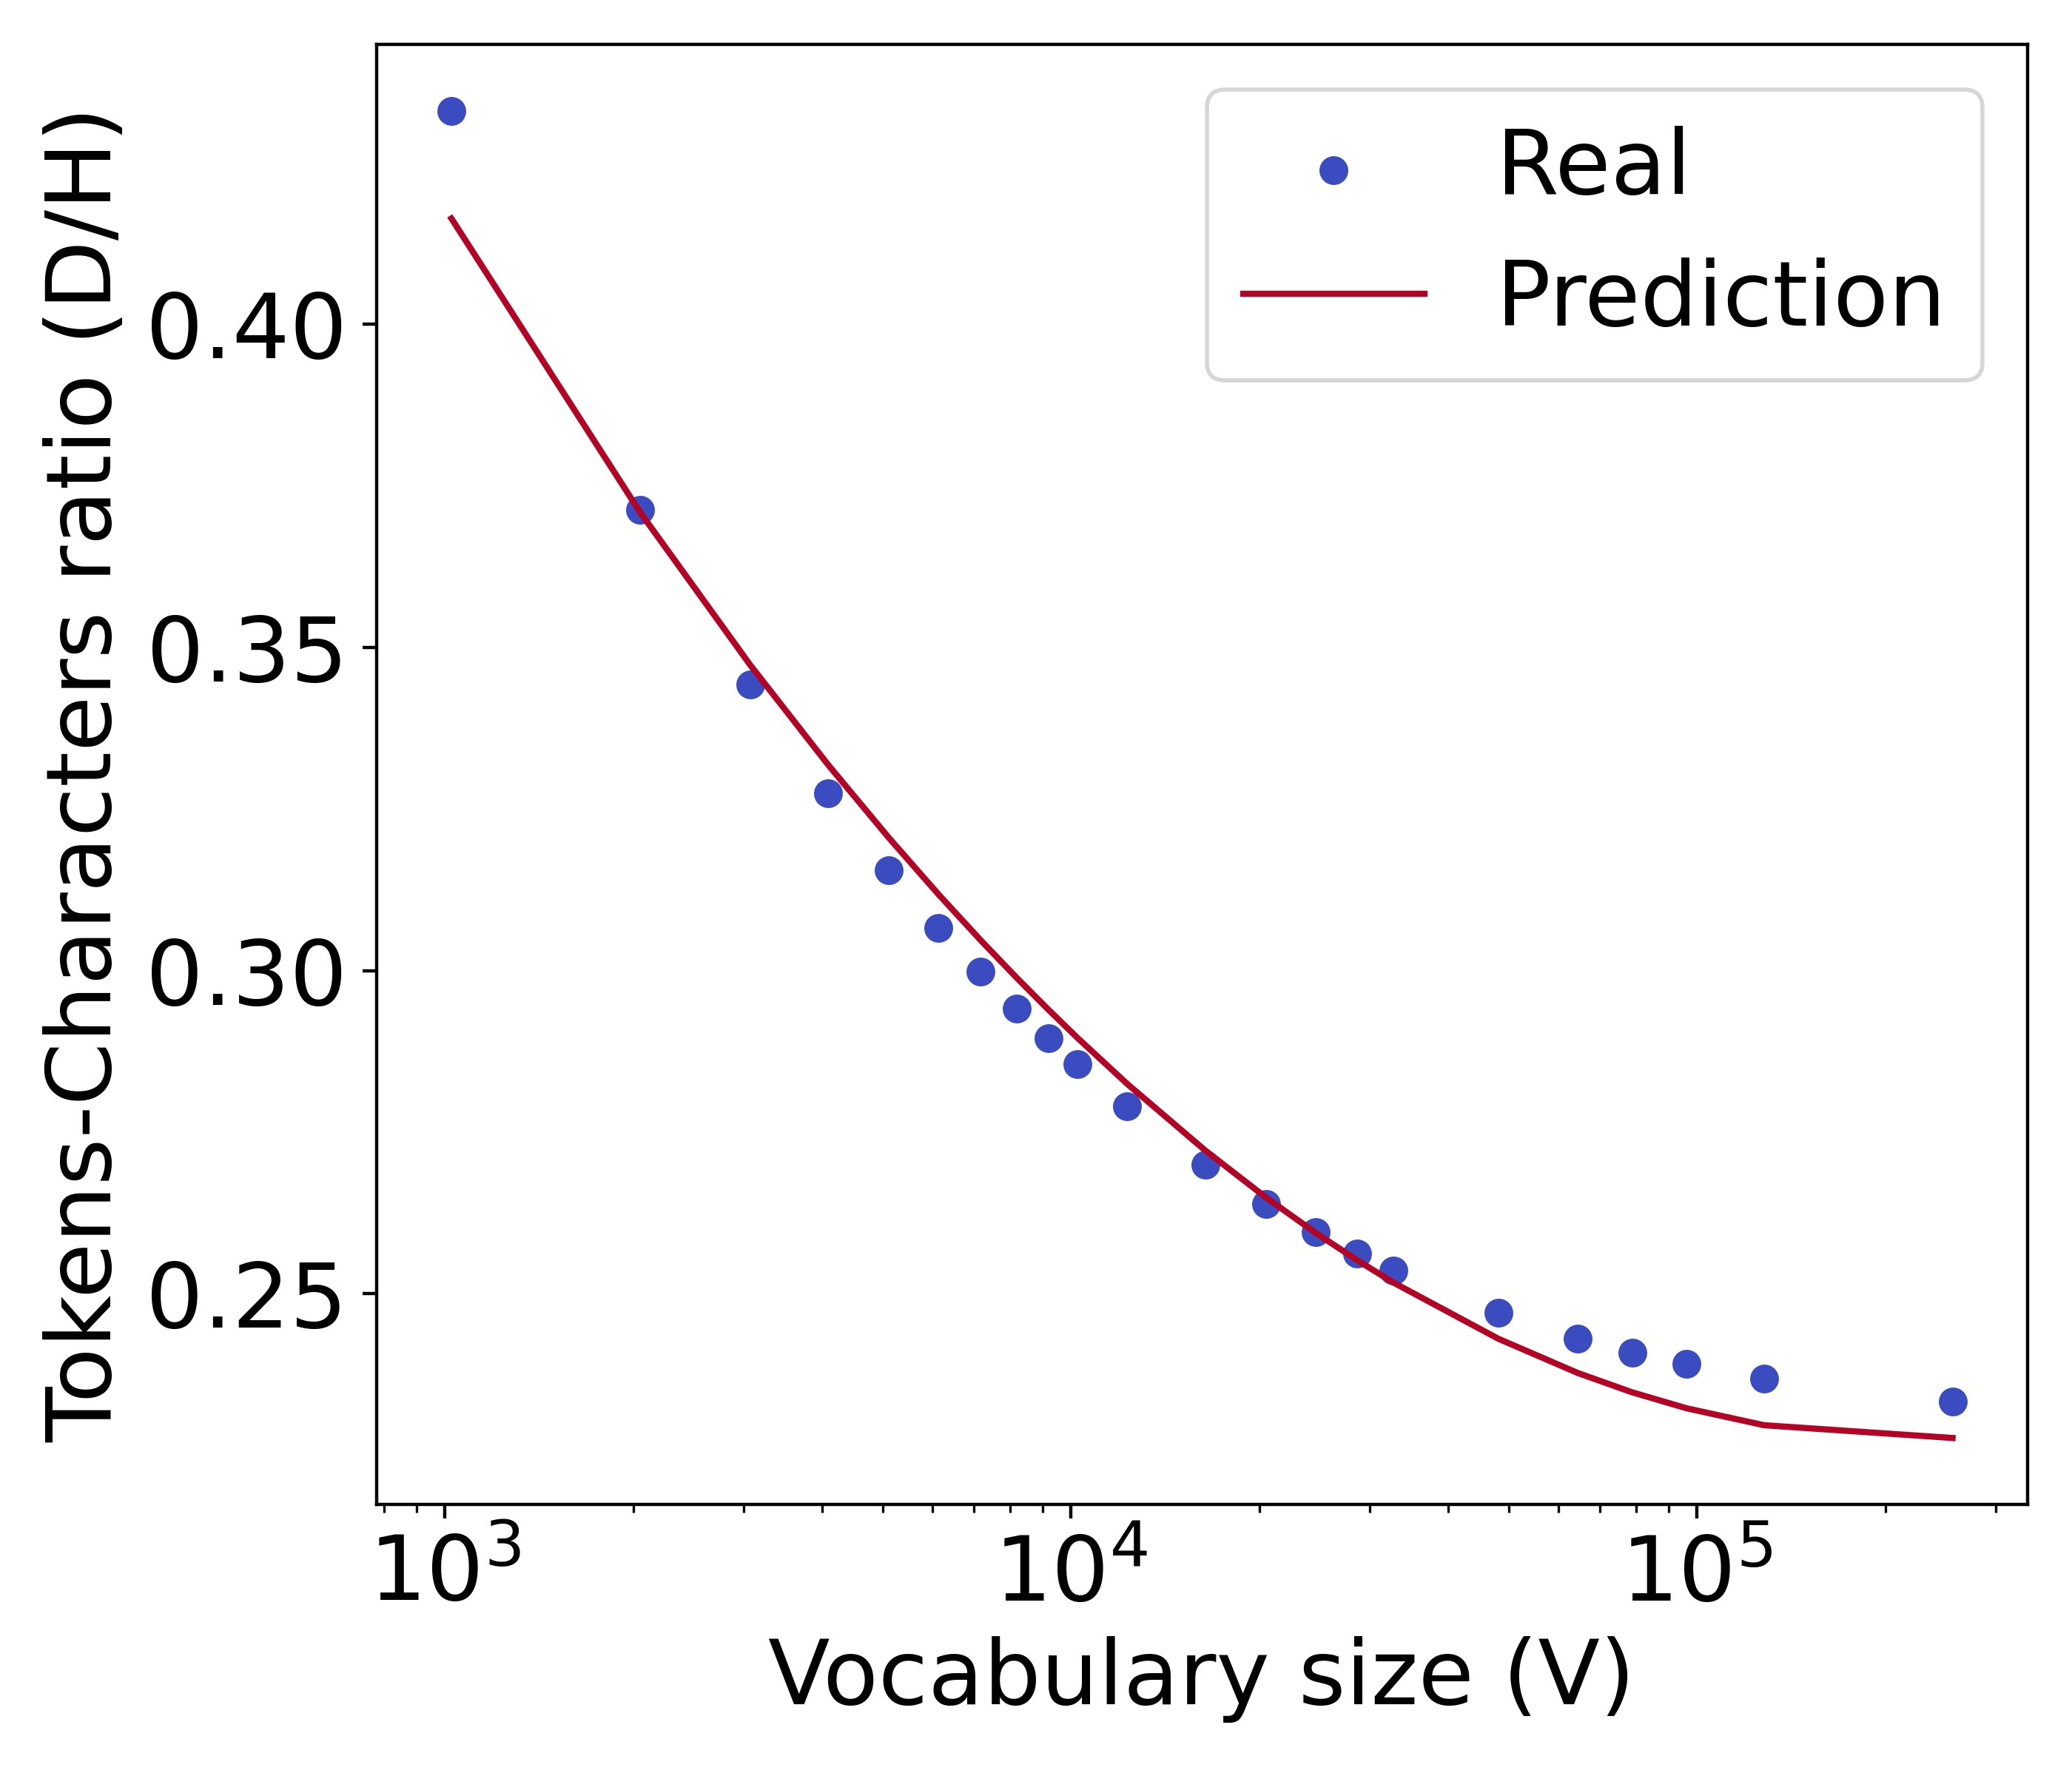
\includegraphics[width=\textwidth]{figures/fit_slimpajama_rmse_0.000376_r2_0.986944_bpe.png}
    \caption{BPE tokenizer\\$RMSE$=3.8e-4, $R^2$=0.99}
    \label{subfig:fv-bpe}
\end{subfigure}
\begin{subfigure}[b]{0.32\textwidth}  
    \centering
    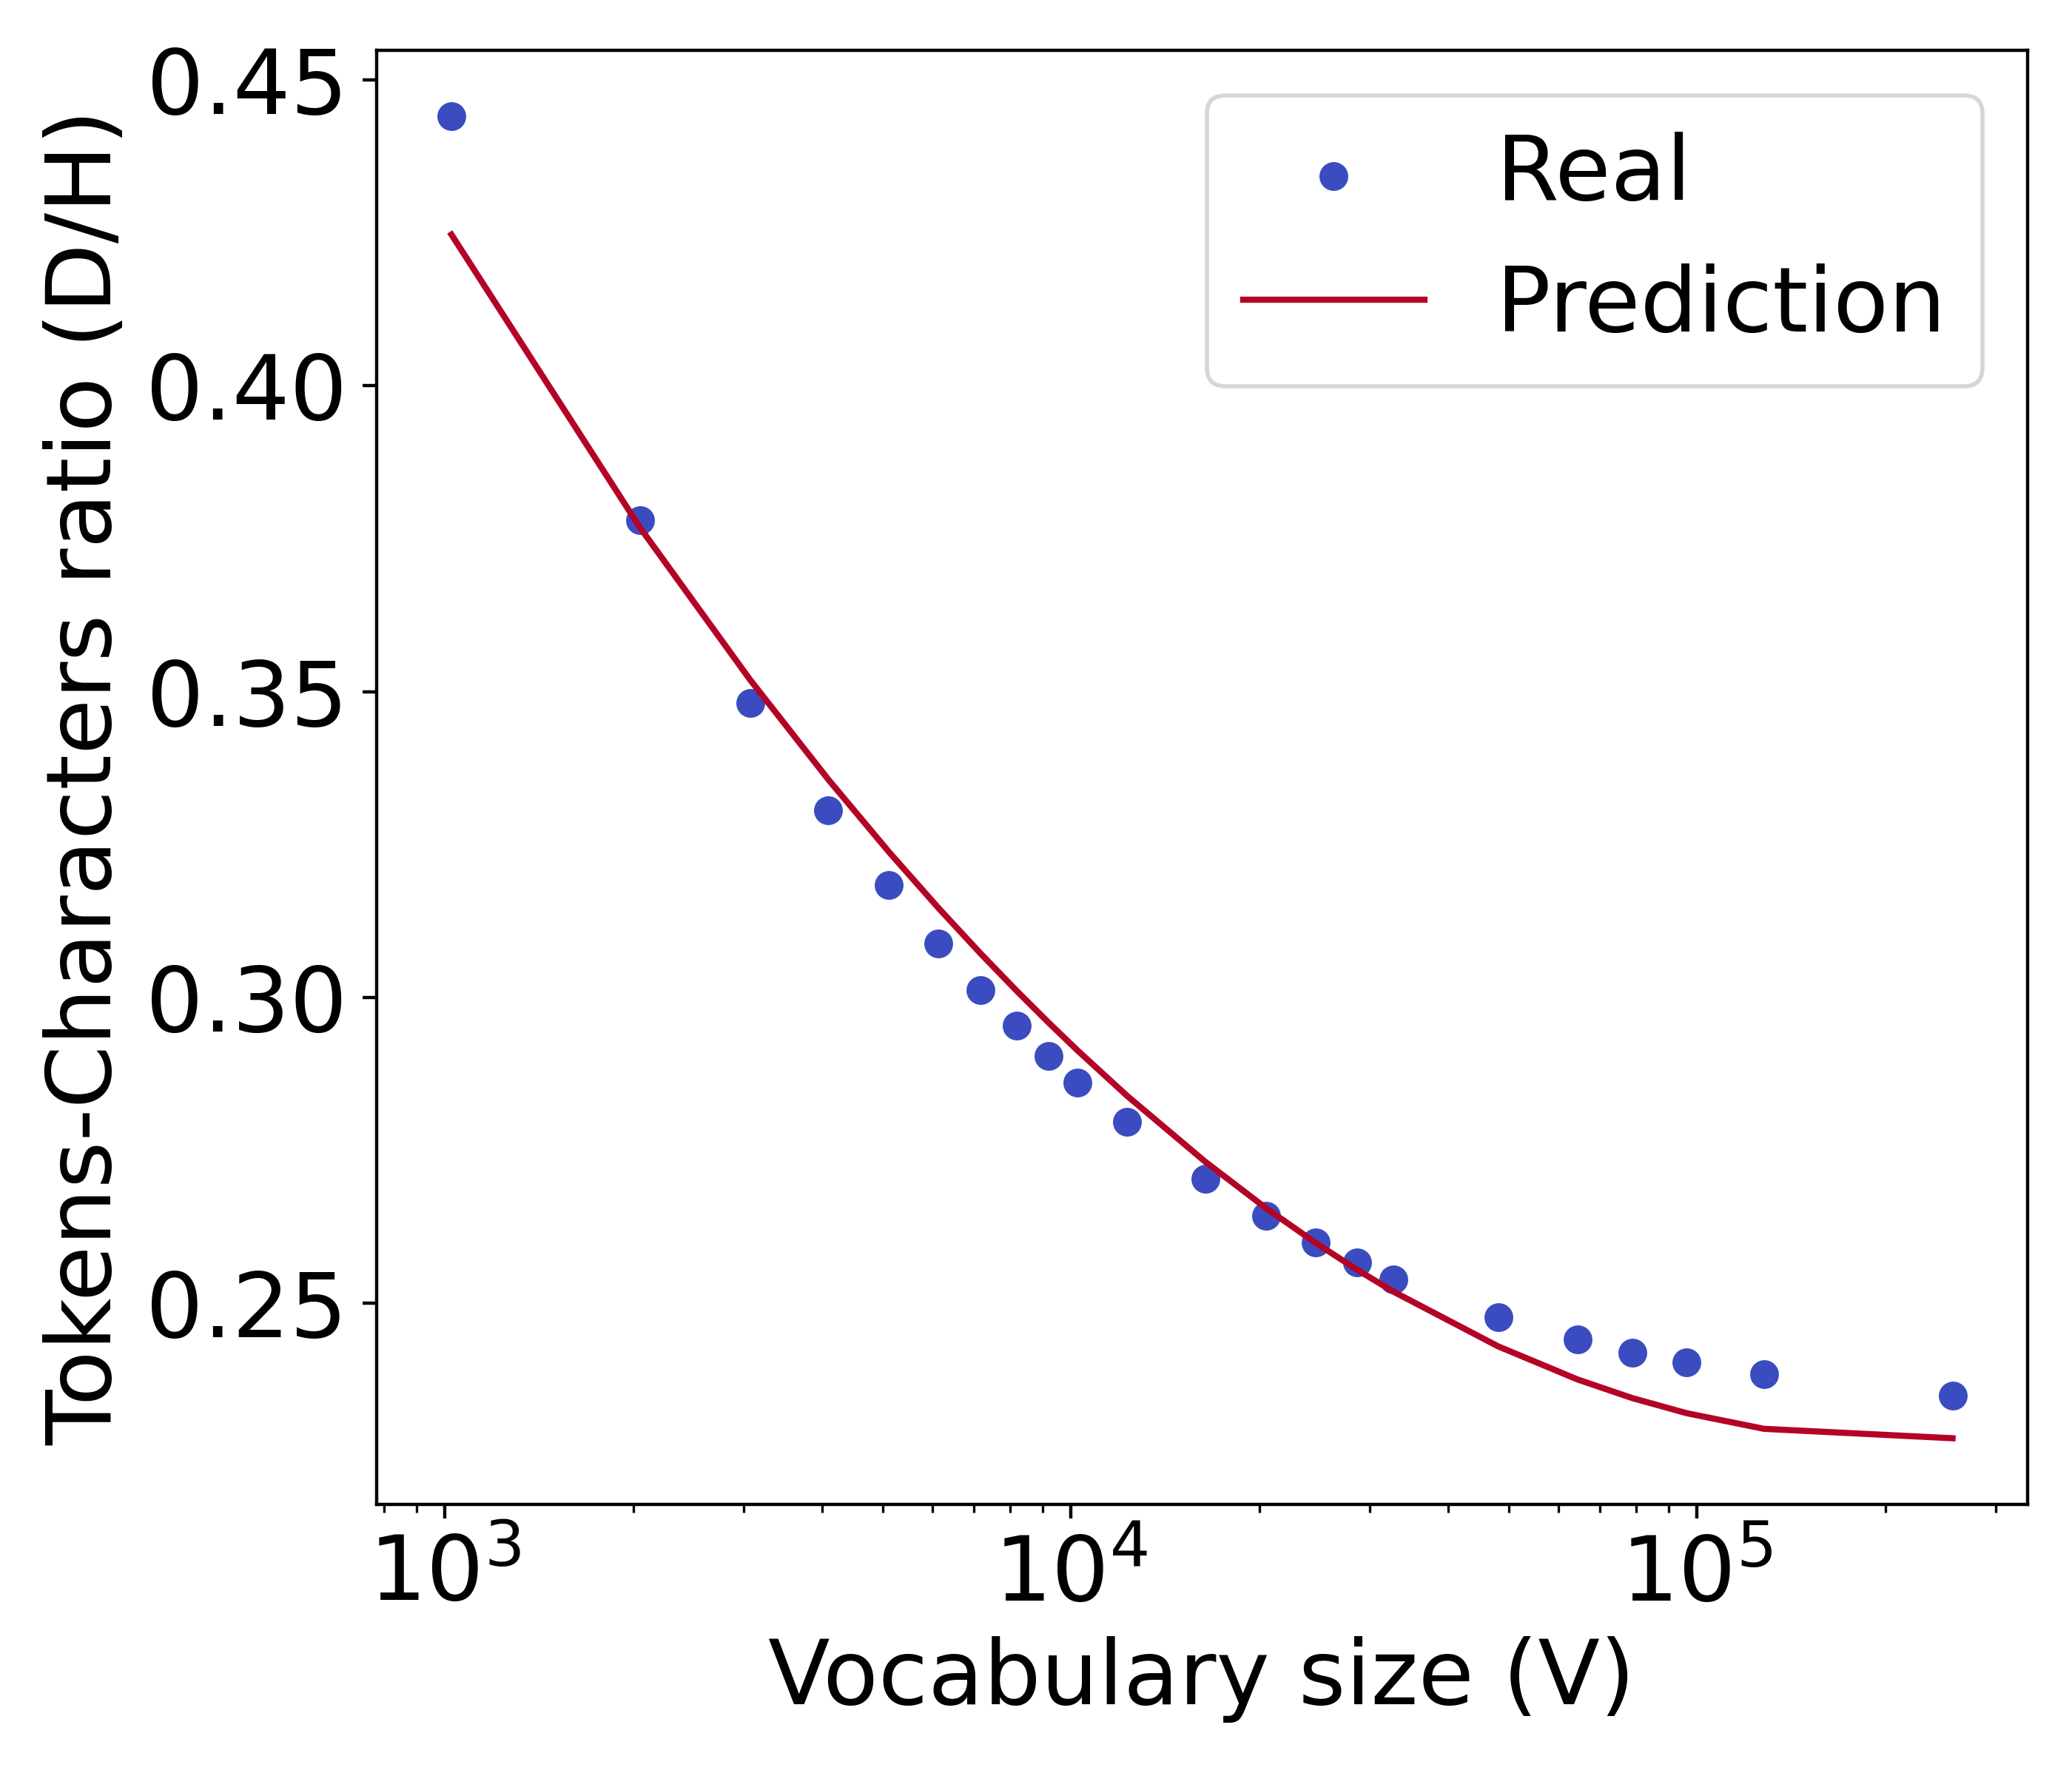
\includegraphics[width=\textwidth]{figures/fit_slimpajama_rmse_0.000524_r2_0.983155_unigram.png}
    \caption{Unigram tokenizer\\$RMSE$=5.2e-4, $R^2$=0.98}
    \label{subfig:fv-unigram}
\end{subfigure}
\begin{subfigure}[b]{0.32\textwidth} 
    \centering
    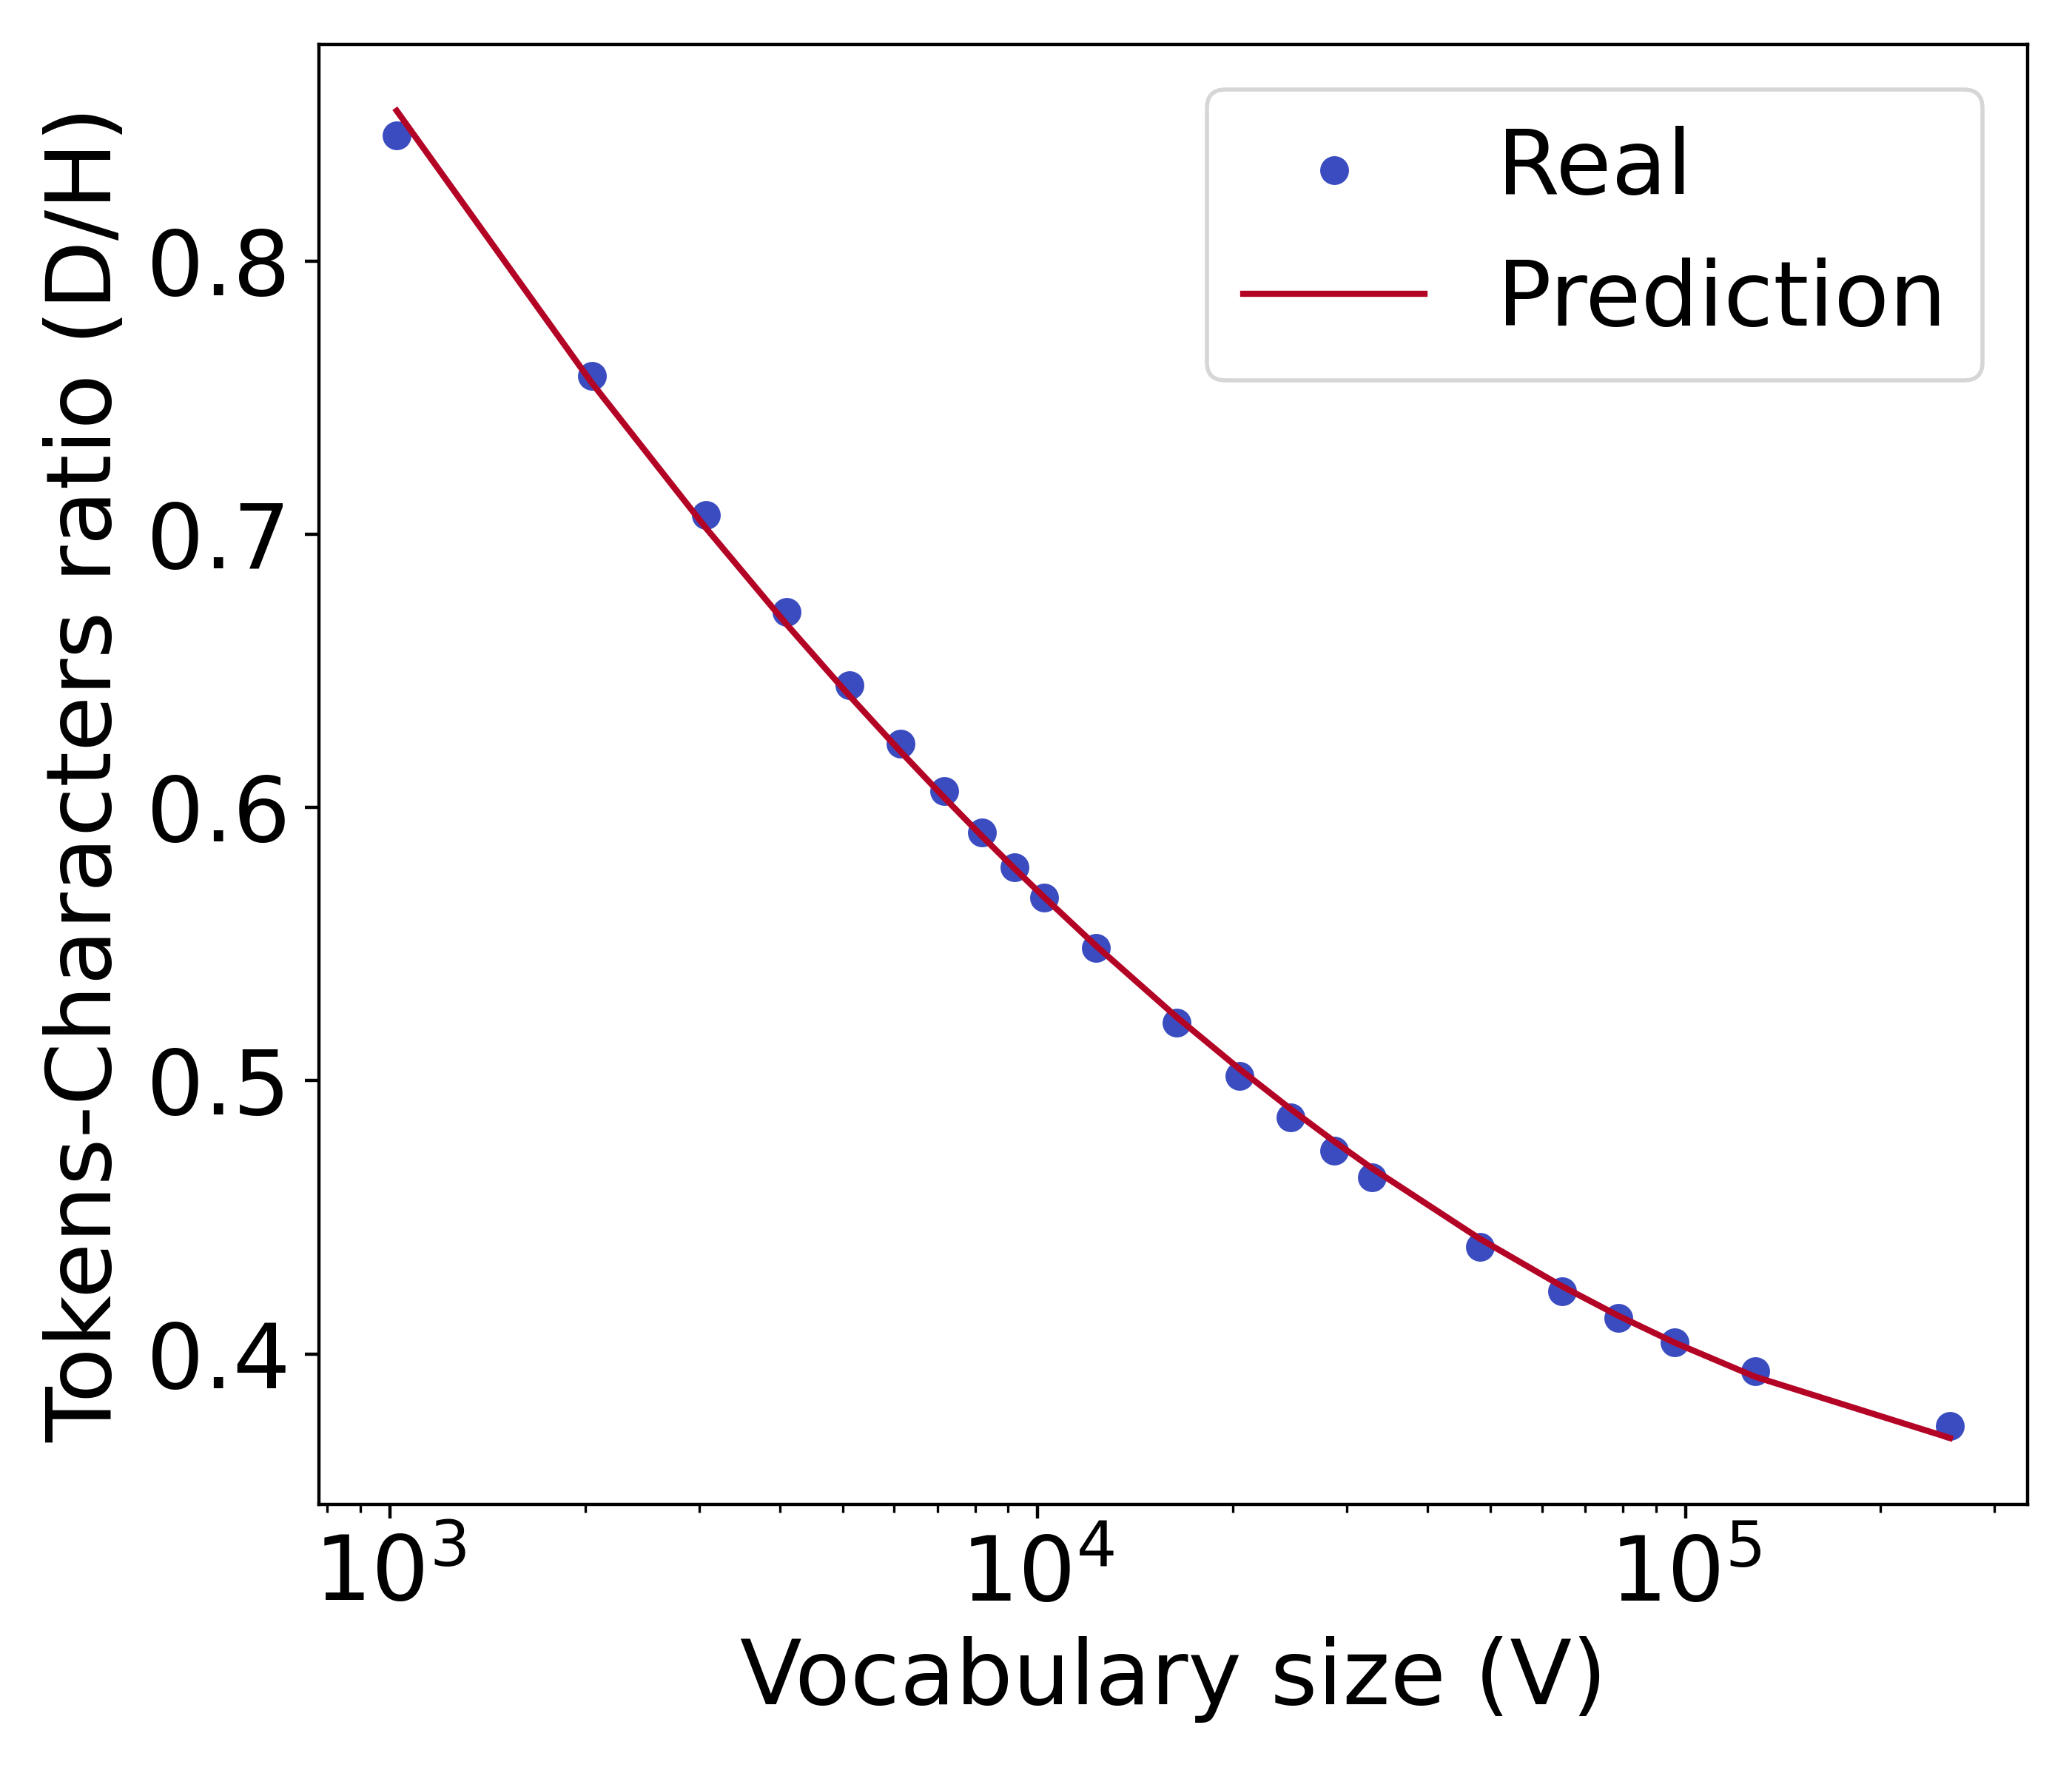
\includegraphics[width=\textwidth]{figures/fit_slimpajama_rmse_0.000036_r2_0.999291_word.png}
    \caption{Word-based tokenizer\\$RMSE$=3.6e-5, $R^2$=0.99}
    \label{subfig:fv-word}
\end{subfigure}
\caption{The modeling of function $f(V)$ with different tokenizers. RMSE and $R^2$ denote the relative mean square error and coefficient of determination, respectively.}
\label{fig:fv-more}
\end{figure}


\paragraph{Robustness to the range of the vocabulary size} The quadratic function on the logarithmic value of vocabulary size that we propose can precisely predict the tokens-characters ratio with an RMSE of 1.5e-6 and $R^2$ of 0.99. However, as a quadratic function is single-peaked, increasing $V$ will increase the output value of $f(V) = a \log^2(V) + b\log V + c$ when $V$ is very large, \textit{e.g.} $V>\exp(-b/2a)\approx 218K$ in our case.

Fortunately, when $V$ is sufficiently large, the tokenization fertility improvement of the tokenizer decays sharply, which results in almost no change to the value of $f(V)$. This is because the words in the training corpus can already be effectively covered by the vocabulary list when the vocabulary size is sufficiently large. In this extreme, the tokenization fertility of the corresponding tokenizer is approaching saturation, thus further increasing the vocabulary size will hardly improve the tokenization fertility.

As an example, there are about 2300M characters in the validation set of the Slimpajama corpus. A tokenizer using a vocabulary size of 2$K$ would yield 140$M$ fewer tokens than a 1$K$ counterpart, but the number of tokens only decreases by 0.7$M$ when going from a vocabulary size of 256$K$ to 257$K$. Therefore, we add $min(V, 200K)$ before calculating $f(V)$ to ensure its decreasing nature. According to our prediction, a model with 300$B$ parameters has an optimal vocabulary size of no more than 400$K$ with a sufficient amount of training data. If we need to consider extremely large $V$ in the future, we can train tokenizers with larger $V$ in the process of fitting $f(V)$ to arrive at more precise predictions.

\subsection{Experimental verification on the fairness of the unigram-normalized language modeling loss}
\label{sec:verification}

\begin{figure}[htbp]
\centering
\begin{subfigure}[b]{0.43\textwidth} 
    \centering
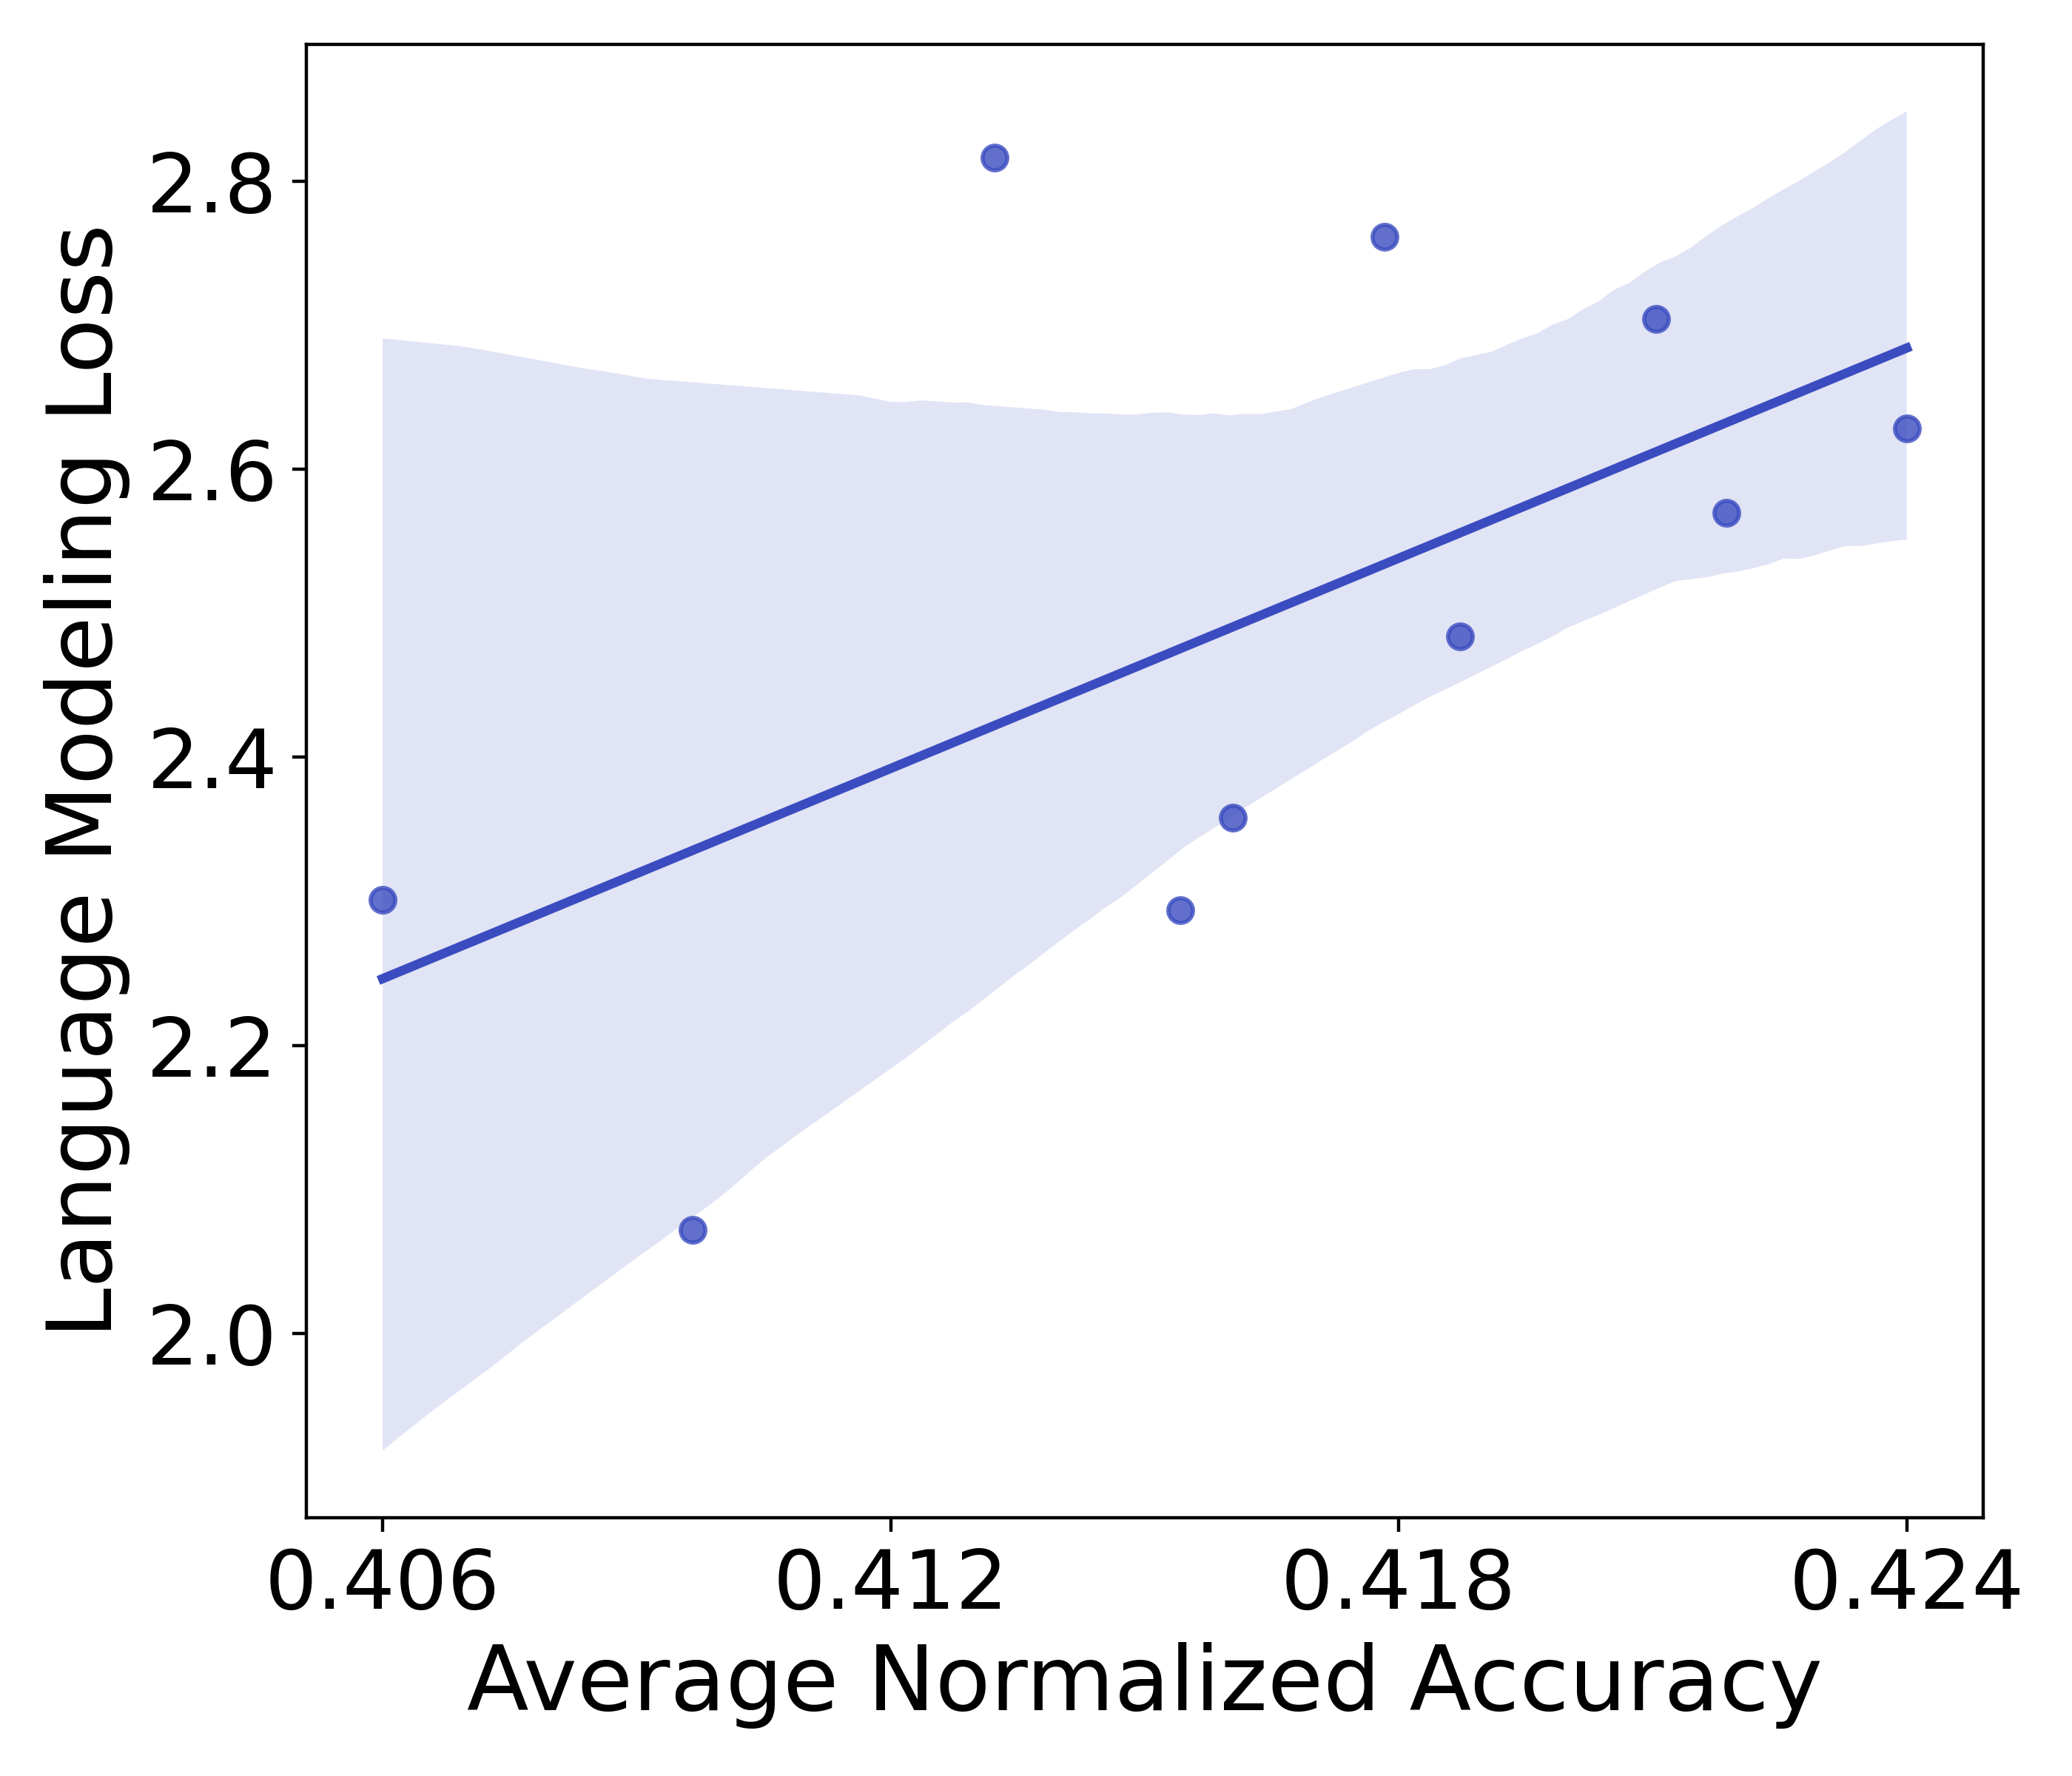
\includegraphics[width=\textwidth]{figures/metric_analysis_loss_corrcoef0.57.png}
    \caption{Relationship between downstream task performance and the commonly-used language modeling loss.}
    \label{loss-accnorm}
\end{subfigure}
\hfill
\begin{subfigure}[b]{0.43\textwidth} 
    \centering
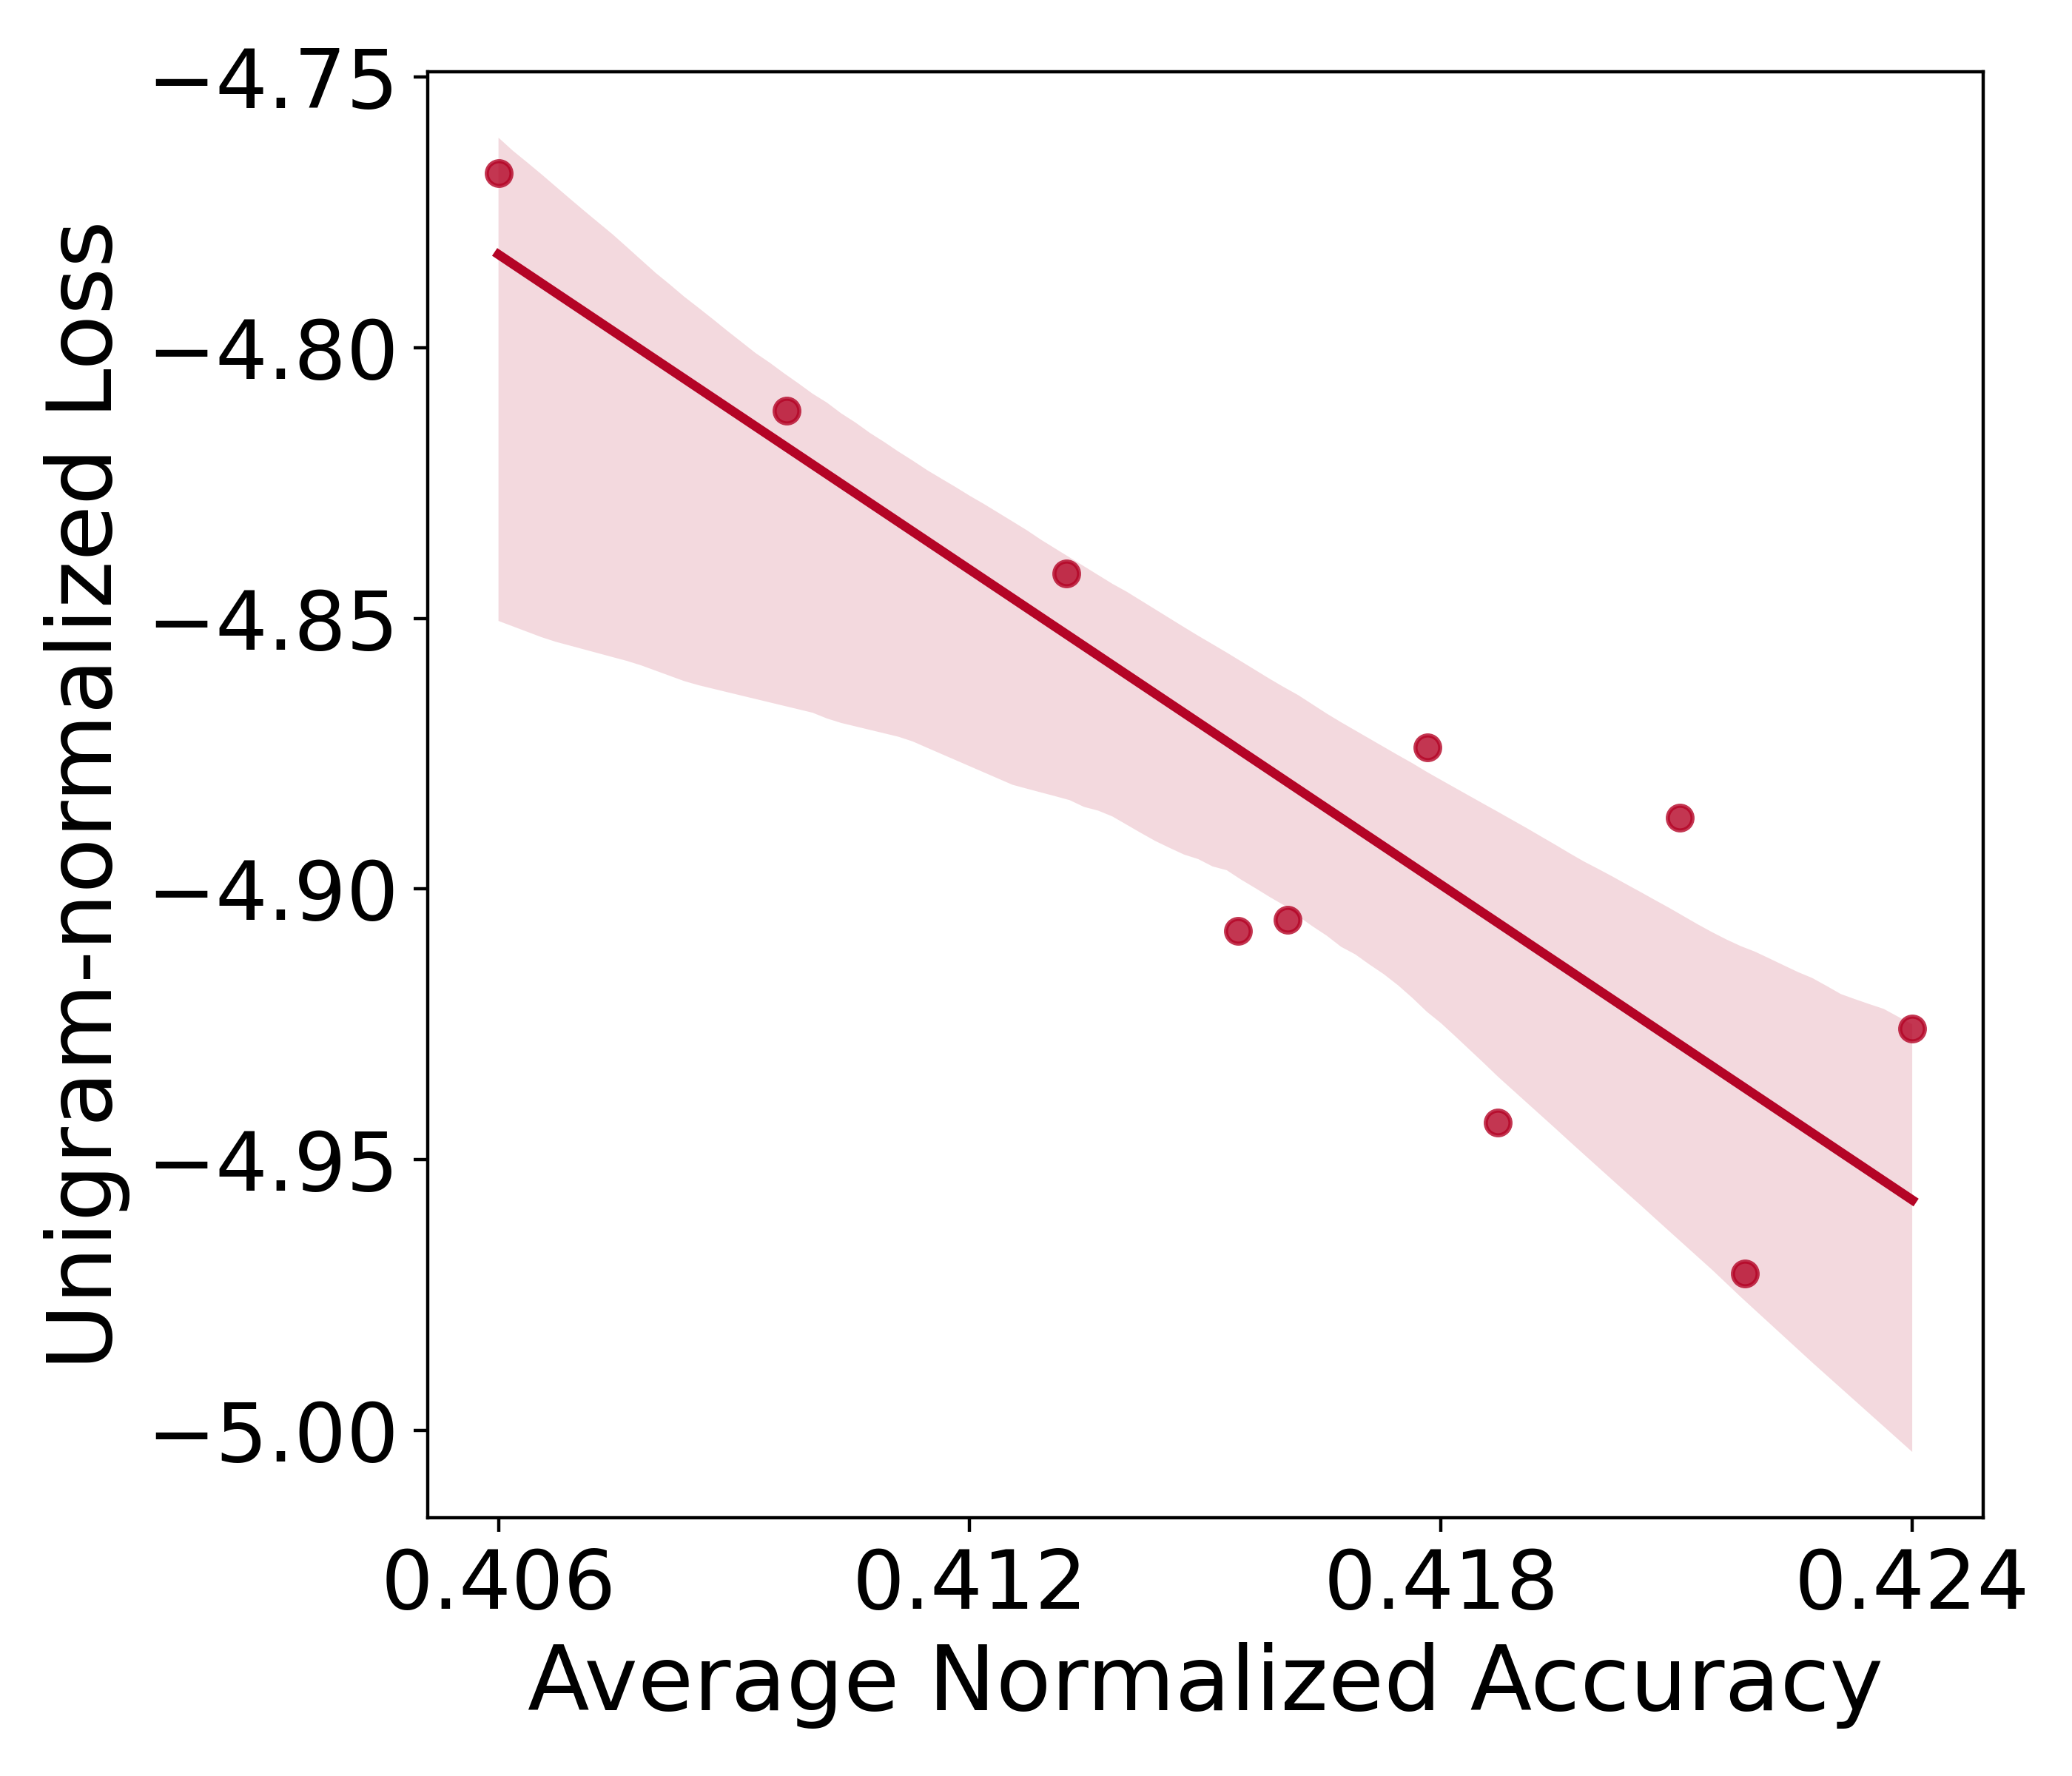
\includegraphics[width=\textwidth]{figures/metric_analysis_lossu_corrcoef-0.88.png}
    \caption{Relationship between downstream task performance and the unigram-normalized language modeling loss.}
    \label{lossu-accnorm}
\end{subfigure}
\caption{
Empirical examination of the fairness of our unigram-normalized loss, $\mathcal{L}_u$. Dots correspond to trained models with varying vocabulary size. We plot their losses (y-axis) and performance on 7 downstream tasks (x-axis): WG \citep{sakaguchi2021winogrande}, PIQA \citep{bisk2020piqa}, OBQA \citep{mihaylov2018can}, Hellaswag \citep{zellers2019hellaswag}, BoolQ \citep{clark2019boolq}, ARC-E \citep{clark2018think} and ARC-C \citep{clark2018think}. The straight line reflects the results of the regression fit with the shade indicating the confidence interval.
}
\label{fig:preparation}
\end{figure}


In \autoref{sec:preliminaries}, we have explained that we use a unigram-normalized loss, $\mathcal{L}_u$, to fairly evaluate models that vary in vocabulary size. Here we empirically verify this choice. We train models with a fixed number of non-vocabulary parameters $N_{\rm nv}$ and embedding dimension $d$ but varying vocabulary sizes $V$. Thus, their vocabulary parameters $N_v$ also vary. We plot the final language model loss and unigram-normalized loss of these models compared to downstream performance in \autoref{fig:preparation}. The language modeling loss exhibits a positive correlation with downstream performance: Models with a higher language modeling loss have better downstream performance. This is because our models with larger vocabularies naturally have a higher loss due to the objective function, yet they can be actually better models with better downstream performance. Our unigram-normalized loss solves this problem and exhibits the expected negative correlation between loss and downstream performance: a lower loss comes with better downstream performance. This empirically justifies our use of $\mathcal{L}_u$ throughout this work.

\subsection{Prediction for Llama3}

While our primary experiments focus on the Llama2 vocabulary size, we also extend our conclusions to Llama3, predicting its optimal vocabulary under optimal compute allocation. As shown in \autoref{fig:scaling-llama3}, we provide detailed predictions for various sizes of Llama3 models. Although Llama3 significantly increases its vocabulary size from 32K to 128K, our research suggests that this may still be insufficient for the larger model sizes of 70B and 400B.

\begin{figure}
    \centering
    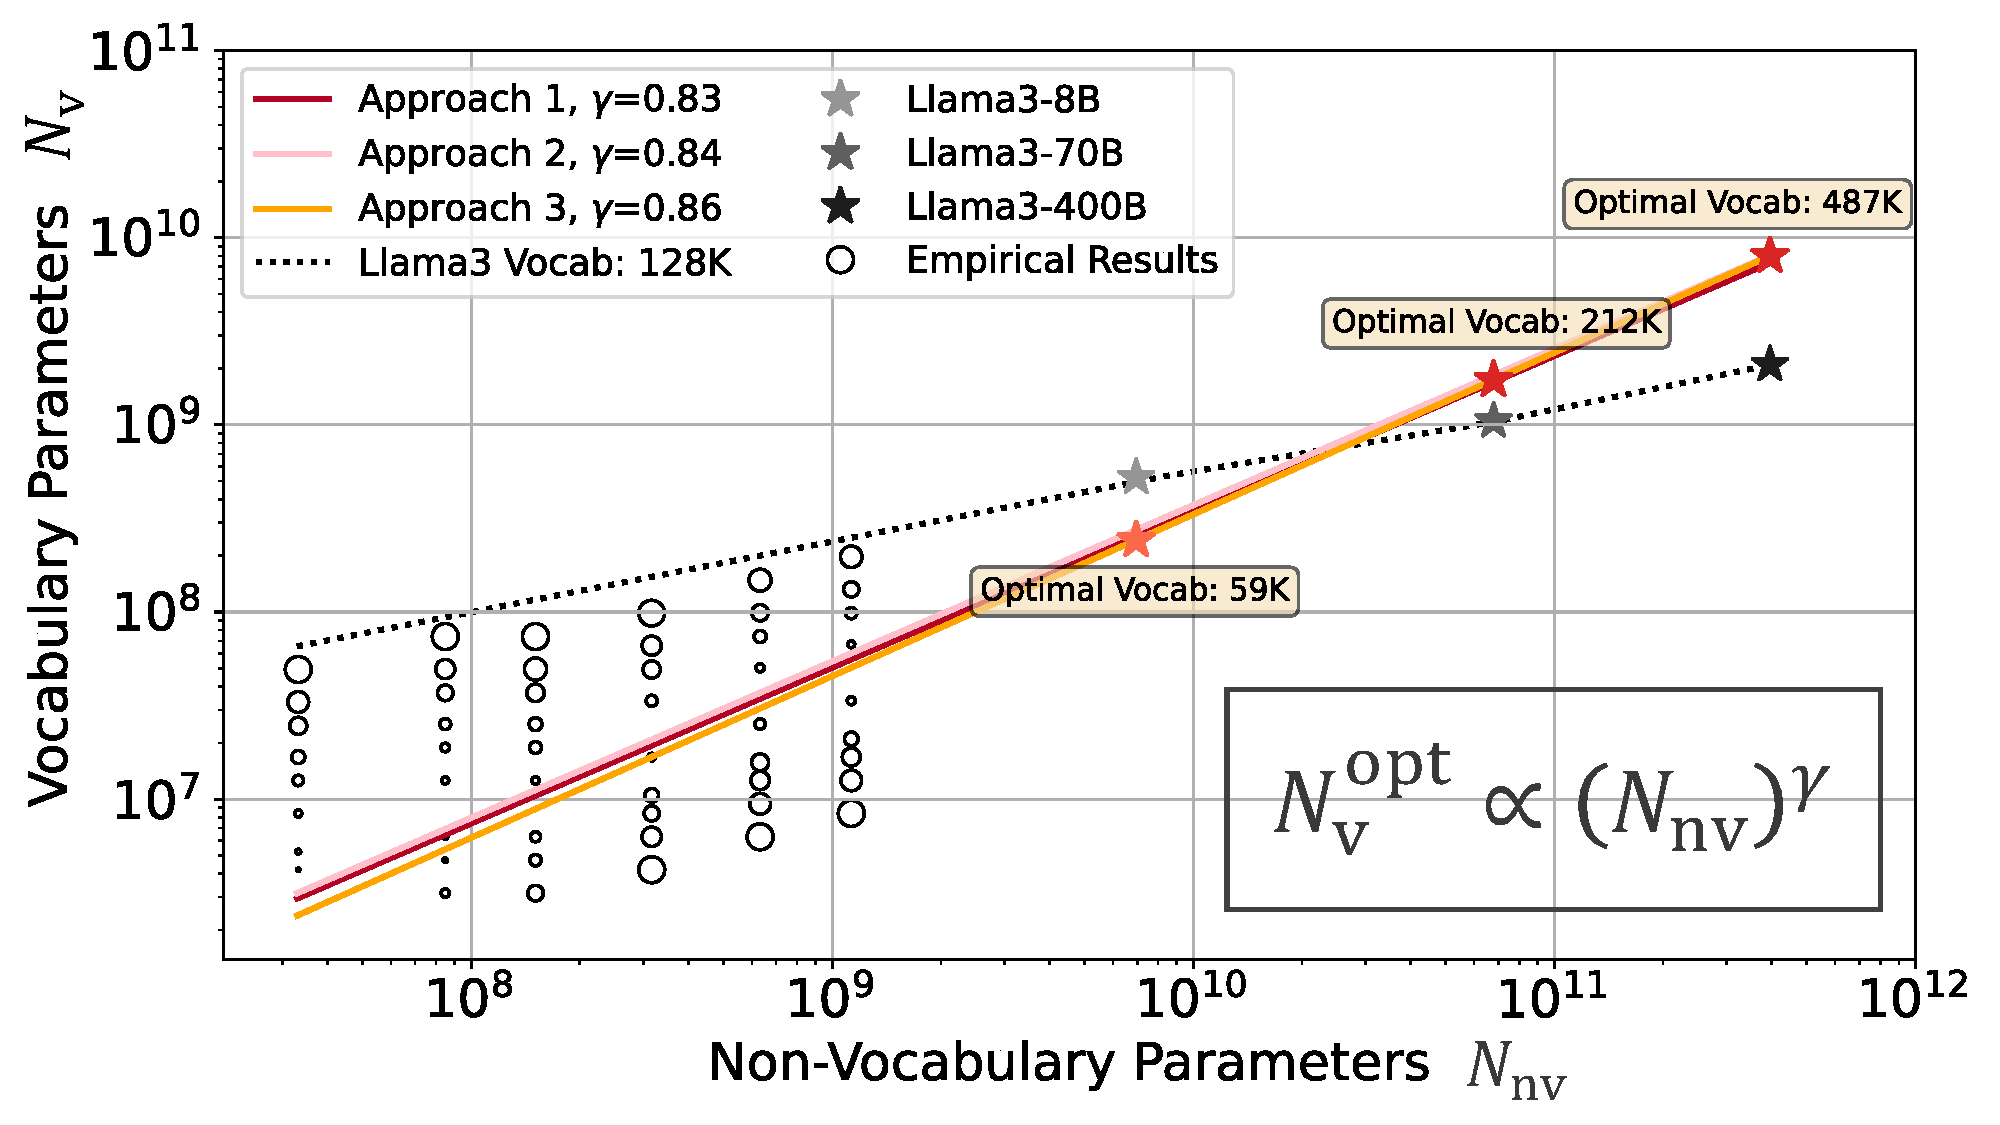
\includegraphics[width=0.95\textwidth]{figures/scaling-llama3.pdf}
    \caption{The replication of \autoref{fig:intro} for Llama3. As shown, the predicted optimal vocabulary size for the Llama3-400B model is as high as 487K.}
    \label{fig:scaling-llama3}
\end{figure}

\subsection{More Related Work}

\paragraph{Vocabulary in language models} The vocabulary of a language model influences its performance significantly~\citep{takahashi2017neural,wang2019improving,xu2020vocabulary}. A larger vocabulary size helps cover more words thus reducing the likelihood of out-of-vocabulary (OOV) cases~\citep{enarvi2017automatic}. \citet{takahashi2017neural} find that larger vocabularies are better at capturing the true statistical distribution of language.
Similarly, expanding vocabulary in multilingual models~\citep{wang2019improving,chung-etal-2020-improving,zheng-etal-2021-allocating,liang-etal-2023-xlm} improves performance, especially for low-resource languages.
However, large vocabularies~\citep{le2023bloom} increase the computational overhead during both training and generation phases.
For example, \citet{liao2021efficient} demonstrate that low-frequency words often lack sufficient examples to develop robust representations when vocabularies are excessively large.
\citet{dou2024sailor} reveal that expanding vocabularies during continual pre-training can lead to significant performance degradation for low-resource languages.
More recently, \citet{dagan2024gettingthemost} explored the trade-offs associated with vocabulary size, proposing optimal vocabulary sizes for both memory efficiency and inference speed in code generation tasks.
Our work complements these efforts by focusing on the broader impact of vocabulary size on downstream performance across various tasks. Specifically, we address a critical, under-explored question: How can we optimally allocate vocabulary size to maximize the downstream performance with the same compute budget?

\paragraph{Byte-level language models}

Recent work has explored byte-level language models~\citep{yu2024megabyte,wang2024mambabyte}, which offer advantages in decoding efficiency and noise robustness compared to token-level models. However, typically limited to parameters under 1B, these models have not been effectively scaled up.
Our scaling laws suggest that the limited vocabulary (i.e., 256 in byte-level language models) may constrain their performance, especially for larger models. The insight provides a potential explanation for the challenges in scaling byte-level models and implies that successful scaling of language models may require proportional increases in vocabulary size.

